\chapter{Physically-Informed Operational Robotic Trajectories for Scientific Expeditions}
\label{chap:phortex}

\begin{center}
    \begin{minipage}{0.7\textwidth}
      \begin{small}
        Now it would be very remarkable if any system existing in the real world could be exactly represented by any simple model. However, cunningly chosen parsimonious models often do provide remarkably useful approximations...For such a model there is no need to ask the question "Is the model true?". If "truth" is to be the "whole truth" the answer must be "No". The only question of interest is "Is the model illuminating and useful?".\\ \emph{George Box}
      \end{small}
    \end{minipage}
    \vspace{0.5cm}
\end{center}


On expeditions, quality observations of water column properties and their anomalies are strong evidence used by a science party to strategically plan research activities---deployment of certain instrumentation or platforms (where, when, why), allocation of resources to different projects, and scheduling for high-stakes one-off missions. In \cref{chap:afar}, we show how to parse scientific instrumentation data for hydrothermal plume identification by domain experts to assist in data discoverability and interpretation. These tools provide descriptive snapshots of what was observed during a mission, but rely on the science experts to extrapolate these snapshots into future mission states. In this chapter, we directly address how to recover a predictive model of plume state from partial observations collected from heterogeneous sensors, and formulate an automated routine for leveraging this predictive model to design dense charting surveys with AUV \Sentry. Content from this chapter is directly adapted from~\cite{preston2022physically}.

\section{Introduction}
Transient, dynamic phenomena---deep-sea hydrothermal plumes, algal blooms, warm core eddies, lava flows---are of interest in many disciplines of observational science. \emph{Expeditionary science} encapsulates the observational sciences that require \emph{in situ} sample collection of environmental phenomena for scientific discovery and model development. In such cases, the environmental targets are typically impossible to observe using remote sensing (e.g., satellites) either due to desired spatial and temporal resolution, environment adversity (e.g., the deep sea, within closed structures), or the nature of the scientific target of interest and corresponding sensing equipment (e.g., building a taxonomy of algae requires physically processing water samples). Expeditionary science is, by definition, conducted in partially-observable and often dynamic environments; thus performing useful and effective data collection in expeditionary science poses a challenge for human and autonomous decision-makers alike.

In this chapter, we study a particular problem within the expeditionary sciences: mapping the space-time dynamics of deep-sea hydrothermal plumes using an autonomous mobile robot. Deep-sea hydrothermal plumes are a source of chemicals and particulates that play a significant role in biogeochemical cycling in the deep ocean\autocite{le2019hydrothermal,resing2015basin,dick2013microbiology, vic2018dispersion, scholz2019shelf}. Understanding the fate of chemicals and particulates in hydrothermal plumes is of significant interest to biogeochemists and physical oceanographers; however, directly studying plumes in the water column is a substantial challenge. Chiefly, deep-sea plumes have complex dynamics in space and time---advective forces (e.g., deep currents, topographic updrafts), diffusion, and turbulent mixing act on plumes as they rise through the water column. A robot tasked with charting a plume must be able to forecast where and when it will intersect with different regions of the plume in order to collect useful observations of its spatiotemporal structure, but the underlying dynamics of a plume are uncertain as these forces are generally unobserved. The problem is exacerbated by the inherent challenge of sensing a plume using chemical sensors --- the chemical distribution of a plume can only be observed with point sensors and no single point measurement is sufficient to locate the plume.

In addition to the technical challenges of determining a sensing strategy for a highly uncertain and dynamic phenomena, the deep-sea environment ($>$\SI{200}{\meter} depth) can only be accessed by depth-capable equipment that are often significantly constrained by operational and safety policies. For example, autonomous underwater vehicles (AUVs) in this setting are typically restricted to execute preset trajectories hand-designed by human scientists\footnote{e.g., \autocite{camilli2010tracking}}. In this mode, the AUV cannot react to measurements while executing the set trajectory. Such ``open-loop'' trajectories can result in sparse measurements of a target phenomenon, such as a dynamic plume, or can miss short-lived events entirely\autocite{flaspohler2019information, preston2019adaptive}. However, this open-loop concept of operations remains the state-of-the-art in practical deep-sea science because preset trajectories are easy to encode, do not require extensive on-platform computing resources, and result in predictable robot actions that can easily be supervised. Here, we consider constraints introduced by a specific robot, the AUV \emph{Sentry}. \Sentry is operated by the National Deep Submergence Facility (NDSF) at the Woods Hole Oceanographic Institution (WHOI)\autocite{kaiser2016design} and by operational policy is only permitted to execute pre-determined regular trajectories like ``lawnmower'' patterns or spirals, making online adaptation impossible. %However, given the cost of scientific field operations and the value of the data collected, it is critical to improve the efficacy of robots like \Sentry as scientific tools. 

Enabling depth-capable robots such as \Sentry to perform expeditionary science and study spatiotemporal phenomena using preset, non-adaptive behaviors requires an autonomy system that can design fixed trajectory patterns strategically to maximize desirable intersections with a dynamic phenomena. To strategize effectively, this autonomy system should learn to forward simulate the dynamics of the target environment over a long-horizon from a small history of robot deployments and plan subsequent deployments using these predictions. This is fundamentally a \emph{sequential decision-making problem}, and is closely related to informative path planning (IPP) problems, in which a robot selects behaviors according to an information-theoretic reward function using a probabilistic belief of the environment. Existing methods in IPP\footnote{e.g., \autocite{Hitz2017,hollinger2013sampling,flaspohler2019information,levine2010information,binney2012branch}}, the related field of experimental design and optimal sensor placement\footnote{e.g., \autocite{krause2008near,wang2019reinforcement}}, and general decision-making under uncertainty\footnote{e.g., \autocite{sunberg2018online, somani2013despot,kocsis2006bandit,Silver2010}} have demonstrated that sequential decision making can be applied to sampling scenarios in which online, adaptive behaviors are possible, the phenomenon of interest is static, and/or there is an opportunity to train the belief model from many trials, multiple sensors, or highly adaptive trajectories. Each of these typical scenarios is violated for the expeditionary science sampling problem, and in this paper we propose an autonomy framework, \PHORTEX: \phortex, that addresses each of these constraints with the set of algorithmic choices made for the observational model, belief representation, and planner within the framework (\cref{fig:intro_summary}). 


\begin{figure}[h!]
    \centering
    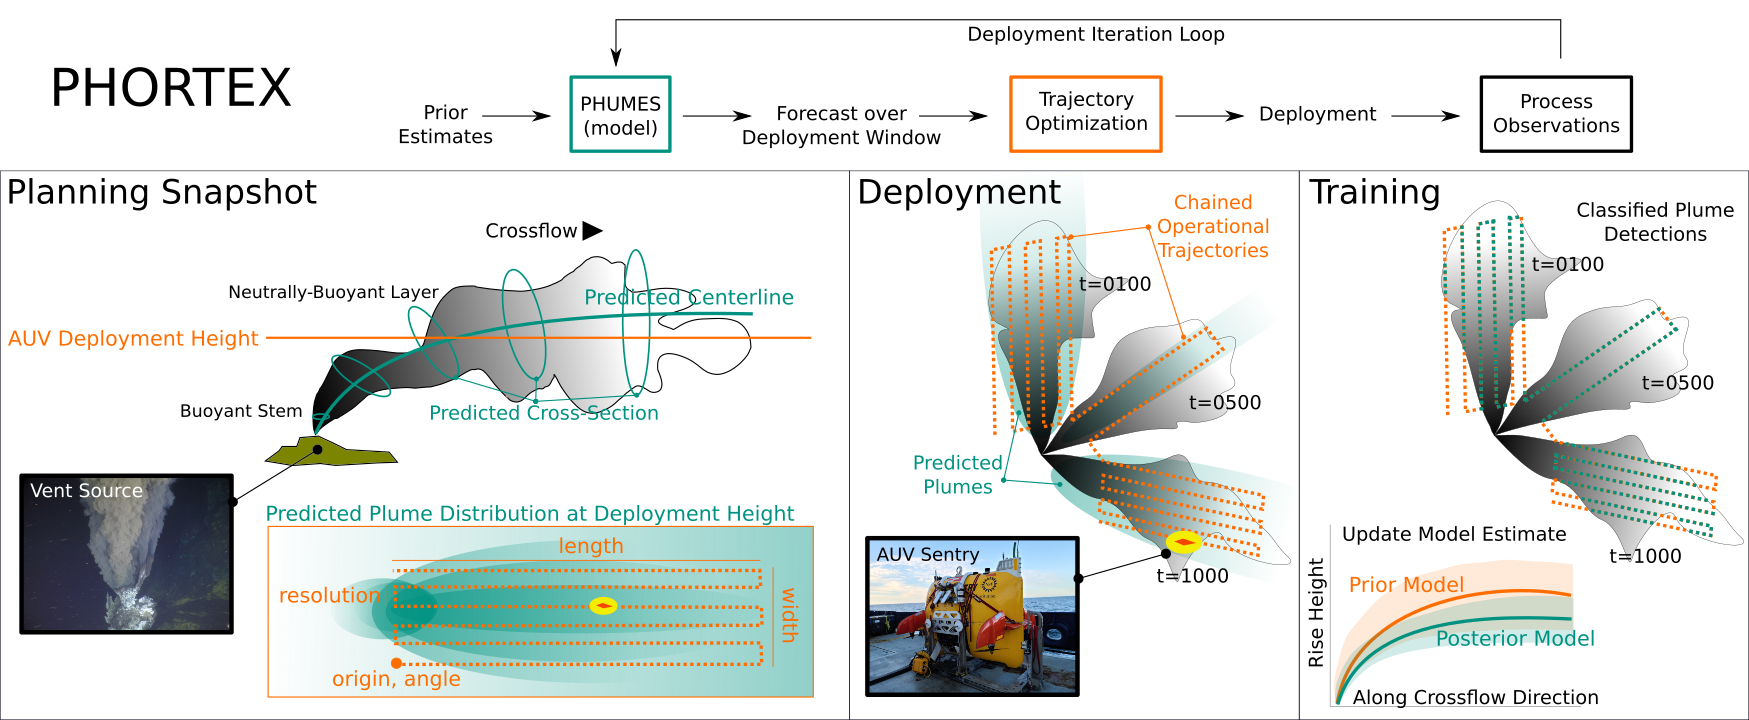
\includegraphics[width=\columnwidth]{figures/summary_intro_figure.png}
    \caption{\textbf{An overview of \PHORTEX: \phortex.} Over the course of an expedition, an autonomous vehicle is deployed several times. In preparation for a deployment, the belief model \PHUMES: \phumes is used to generate a probabilistic forecast of the target spatiotemporal distribution. \PHUMES can be seeded with prior information from scientific knowledge, data of opportunity from other deployed sensing equipment, or previous robot deployments. A trajectory optimizer is given the forecasts and modifies the parameters of a trajectory primitive. Several primitives are chained together to form a complete deployment trajectory. The robot is then deployed and executes the trajectory. Following a deployment, \emph{in situ} observations from multiple heterogeneous science sensors are collected from the robot and fused into a data product that can be used to train \PHUMES, and the deployment planning process iterates. Here, the task of hydrothermal plume charting with AUV \emph{Sentry} is illustrated. \PHUMES generates a forecast of temporally-evolving plume centerlines and cross-sections from estimates of vent characteristics and fluid crossflow (e.g., current) informed by measurements or prior distributions over these variables. For a given height that \emph{Sentry} can operate (and is constrained to operate for any given primitive), chains of uniform coverage lawnmowers are optimized (over parameters such as height, width, origin, and global angle) with respect to the plume forecast to intersect and track the plume over the course of a deployment window. Following a \emph{Sentry} deployment, observation locations are classified as binary plume detections from analysis of several science sensors. This product is then used to update the \PHUMES model of plume centerline and cross-section over time. The new \PHUMES model is then used to plan the next deployment of \Sentry.}
    \label{fig:intro_summary}
\end{figure}


%%%%%%%%%%%% Contributions
\subsection{Contributions}
In this chapter, we formulate our autonomy stack \PHORTEX to solve the hydrothermal plume charting problem under operational constraints imposed by a state-of-the-art AUV, \Sentry. \Sentry, by policy, can only execute pre-defined trajectories while underway, and can only be deployed a small number of times during a given expedition. As modern IPP, plume-hunting, and front-tracking techniques strongly rely on underway adaptive behaviors, we extend these frameworks for \Sentry by formulating a \emph{deployment-by-deployment} sequential decision-making problem which treats each pre-defined deployment of \Sentry as a single action in sequence with few steps. We define each deployment action as a chain of operationally-approved trajectory primitives (i.e., lawnmower patterns), which are parameterized by a small number of characteristics including their relative size, resolution, and position, and are optimized to collect the most number of expected in-plume detections.

To represent the robot's knowledge (belief) in order to optimize a given chain for tracking a target plume, we introduce a probabilistic model \PHUMES: \phumes, which provides long-horizon forecasts of plume state. As very few deployments of AUV \Sentry are possible during an expedition, \PHUMES must overcome the challenge of sample-efficient dynamics learning from sparse, partial observations. To do so, we leverage the existence of well-characterized analytical models for buoyant plume dynamics used in ocean and atmospheric sciences to embed a numerical simulator into a Bayesian filtering framework. The use of this simulator creates a strong inductive bias for the dynamics learning problem for a given field site. There are several advantages to this scheme: the forecasts generated by \PHUMES are driven by a set of physically-meaningful parameters (e.g., vent temperature, crossflow magnitude) which are interpretable by the science team and over which the science team may have useful prior knowledge; the \PHUMES framework can easily accept data or information external to \Sentry deployments that map to the physically-meaningful parameters; and forecasts that are generated support computation of many summary statistics (e.g., mean, variance), providing flexibility for defining reward functions for the trajectory optimization scheme.

Through simulations, we demonstrate that \Sentry using \PHORTEX can collect more spatially and temporally diverse plume-derived fluid samples as compared with classical surveying approaches. The diversity of samples corresponds to observing more unique regions of a plume structure, and has important, positive implications for scientific inquiry to be performed on the dataset collected by \Sentry in post-expedition analyses, to be further discussed in \cref{chap:field_results}. 

The rest of this chapter is organized as follows: in \cref{sec:problem} the hydrothermal plume charting sequential decision-making problem is formally presented as a partially-observable Markov decision process (POMDP) and present \PHORTEX and \PHUMES in \cref{sec:methods}. \cref{sec:experiments} provides a description of a simulated deployment and experimental results are discussed in both \cref{sec:phortex_perform} and \cref{sec:phumes_perform}. In \cref{sec:future} open challenges for robotics in expeditionary science are highlighted, and finally in \cref{sec:conclusion} some closing remarks are provided. 

%%%%%%%%%% Logistics
\subsection{Closing the Loop: Expedition Logistics for Deep-Sea Robotics}
\td{Decide whether to keep this section here, or if it should be offboarded to earlier background chapter.}
Oceanographic research expeditions are an undertaking that requires the coordination and collaboration of a science party, external engineering teams that maintain and operate the scientific equipment used during studies, and the captain and crew aboard a research vessel (on which everyone lives and works during operations). Deep-sea ($>$\SI{200}{\meter} depth) capable robotic platforms used in oceanic research are assets independently maintained from a ship, and typically requested on a per-expedition basis. AUV \Sentry may be deployed on tens of expeditions in a given year, with up to 250 days at sea\autocite{kaiser2016design}. Safety of both people and equipment are held to the highest importance. Further, the critical role of \Sentry in oceanographic research drives the strict operational policies that dictate \Sentry deployments to prevent vehicle loss or damage.

It is with this context that \Sentry deployments are designed by the science party and ultimately approved by the \Sentry engineering team. In a typical workflow, the science party may provide a set of coordinates or waypoints they generate based on bathymetric maps, prior knowledge, or previous data (when available). The \Sentry team design survey trajectories based on these coordinates and respecting basic operational constraints of the vehicle (e.g., speed, minimum/maximum altitude from the seafloor). With approval of the \Sentry team, science party, and captain, the survey is then executed. A single ``dive'' of \Sentry is multiple hours (typically not less than 5 hours, and under 24 hours). At the conclusion of a dive, \Sentry is recovered from the ocean and data products containing hundreds of thousands of point measurements from multiple heterogeneous sensors are made available to the science team within a few hours after \Sentry returns to the deck. Depending on the length of the dive, 12-18 hours of vehicle cycling time (e.g., recharging, instrument maintenance, preparation for the next deployment) are required. Based on the length of an expedition and other ongoing research activities, \Sentry may be deployed only a handful of times.

The complexity of these basic operations for \Sentry alone, in addition to the burden of coordinating several other ongoing scientific projects happening simultaneously, day-to-day operational changes, and unforeseen discoveries and hurdles, make performing ``closed loop science'' with robot platforms a challenge while at sea. For hydrothermal plume monitoring, a combination of sensor streams need to be used to make confident plume detections\autocite{jakuba2007stochastic}, but information about exact tidal state, state of the venting source, and background sea characteristics are typically not provided in these products, and can require fusing data from other instruments deployed on a cruise, if available. The planning challenge is further exacerbated when the design of a new mission requires not just deep analysis of the collected data, but forecasting the implications of those data onto a new day, new site, or new objective. 

Our work aims to alleviate the burden of closing the loop onboard a research vessel for AUV operations by positioning \PHORTEX as a means of generating interpretable phenomenon forecasts informed from diverse data streams and trajectories through those forecasts that can be verified by science party members and approved by \Sentry engineers. Algorithmically, the formulation of \PHORTEX as a sequential decision-making framework produces trajectories which are informed by previous observations, thus literally behaving like a closed-loop controller for robot actions. Through a real field mission to the Gulf of California to chart hydrothermal plumes in the northern Guaymas Basin, we demonstrate how \PHORTEX can be practically deployed for plume charting.

\section{Problem Formulation}
\label{sec:problem}
During scientific expeditions, the objective of a robot is to collect useful measurements, as defined by a given task (e.g., reduce uncertainty over a quantity, find the global optimum in a distribution, track a moving target). For hydrothermal plume charting, the goal is to map or ``chart'' the spatiotemporal structure of a buoyant plume using a dynamically constrained AUV. Such a chart enables scientists to infer relevant scientific properties of generating vents (e.g., chemical flux) and to create detailed models of deep-sea interactions and nutrient cycling. We first describe how general problems in expeditionary science can be formulated as sequential decision-making problems, describe the specific constraints of the AUV \Sentry and how they influence the sequential decision-making problem, and finally present a formal description of hydrothermal charting as a partially observable Markov decision process. 

\subsection{Scientific Expeditions as a Sequential Decision-Making Problem}
Expeditionary science requires a robot to make a sequence of decisions to collect scientifically useful measurements of an unknown, partially-observable spatiotemporal environment under operational constraints. Generally, the expeditionary science decision-making problem can be formulated as a partially observable Markov decision-process (POMDP). Let $\Pi(\cdot)$ denote the space of probability distributions over the argument. A finite horizon POMDP can be represented as tuple: $(\Ss, \A, T, R, \Zz, O, b_0, H, \gamma)$, where $\Ss$ are the states, $\A$ are the actions, and $\Zz$ are the observations. At planning iteration $t$, the agent selects an action $a \in \A$ and the transition function $T: \Ss \times \A \to \Pi(\Ss)$ defines the probability of transitioning between states in the world, given the current state $s$ and control action $a$. The transition function governs both how the state of the robot will evolve, given a chosen action, and the potentially stochastic evolution of the underlying spatiotemporal environment. After the state transition, the agent receives an observation according to the observation function $O: \Ss \times \A \to \Pi(\Zz)$, which defines the probability of receiving an observation, given the current state $s$ and previous control action $a$. The reward function $R: \Ss \times \A \to \reals$ serves as a specification of the task, assigning the states of the world that are useful for a given scientific objective high reward and others low reward. A POMDP is initialized with belief $b_0 \in \Pi(\Ss)$ --- an initial probability distribution over state --- and plans over horizon $H \in \integers^+$ with discount factor $\gamma \in [0, 1]$.

As the robot moves through the world, it selects actions and receives observations. Since the state of the world is not directly observable in a POMDP, the robot maintains a probability distribution over possible states (i.e., belief) and must update this distribution each time it takes an action and receives an observation. Given the transition and observation models, the belief can be updated directly using a Bayes filter \autocite{sarkka2013bayesian}:
\begin{align}
    \tau(b_{t-1}, a_{t-1}, z_t) = b_t
        &\defeq \Pi(S_t \mid a_0, z_0, \dots, a_{t-1}, z_{t-1}, z_t) \\
        &= \Pi(S_t \mid b_{t-1}, a_{t-1}, z_t) \\
        &= \frac{\int_{s \in \Ss} O(s, a_{t-1}, z_t) T(s, a_{t-1}, s')b_{t-1}(s')}{\Pi(z_t \mid b_{t-1}, a_{t-1})}
    \label{eq:bayes_tau}
\end{align}

where $\tau(b,a,z)$ is the updated belief after taking control action $a$ and receiving observation $z$ (Eq.~\ref{eq:bayes_tau}). Unfortunately, \cref{eq:bayes_tau} is often intractable to compute directly and an approximate Bayesian inference procedure is required to represent the belief (e.g., a Kalman filter\autocite{welch1995introduction}, a particle filter\autocite{Silver2010}, or variational methods\autocite{wainwright2002environmental,kucukelbir2017automatic}). 

Due to the stochastic, partially observable nature of current and future states, the realized reward in a POMDP is a random variable. Optimal planning is defined as finding a horizon-dependent policy $\{\pi_t^*: \Pi(\Ss) \to \A\}_{t=0}^{H-1}$ that maximizes expected reward: $\mathbb{E} \Big[ \sum_{t=0}^{H-1} \gamma^t R\big(S_t, \pi_t(b_t)\big) \mid b_0 \Big]$, where $b_t$ is the updated belief at time $t$, conditioned on the history of actions and observations. The recursively defined horizon-$h$ optimal value function $V^*_h$ quantifies, for any belief $b$, the expected cumulative reward of following an optimal policy over the remaining planning iterations: $V_0^{*}(b) = \truemax_{a \in \A} \mathbb{E}_{s \sim b}[R(s, a)]$ and
\begin{align}
     V_h^{*}(b) &=  \max_{a \in \A} \mathbb{E}_{s \sim b}[R(s, a)] + \gamma \int_{z \in \Zz} \Pi(z \mid b, a) V_{h-1}^*(\tau(b, a,z)) \, \text{d}z \hspace{0.6cm} h \in [1, H-1],
    \label{eq:value}
\end{align}
The optimal policy at horizon $h$ is to act greedily according to a one-step look ahead of the horizon-$h$ value function. However, \cref{eq:value} is intractable for large or continuous state, action, or observation spaces and thus the optimal policy must be approximated. Much of the art of practical decision-making uncertainty is making well-designed algorithmic and heuristic choices that enable efficient and robust planning algorithms. In the remainder of this section, we introduce the plume charting POMDP with AUV \Sentry and in \cref{sec:methods}, we describe the specific algorithmic choices that enable \PHORTEX to approximately solve it.  



\subsection{Scientific Decision-Making with AUV \emph{Sentry}}
There are several levels at which an AUV can behave autonomously. At the lowest level, an AUV is given navigation waypoints and executes a closed-loop controller and state estimator to drive to that waypoint; this type of autonomy is commonly implemented and executed on AUV platforms. AUV \emph{Sentry} is capable of autonomously navigating between given waypoints using a closed-loop controller and a state estimator that uses acoustic ranging between the robot and the ship to set latitude, longitude, and depth coordinates. More sophisticated autonomy systems that are aware of scientific objectives can build upon this waypoint controller to enable sophisticated autonomous behavior. 

\textit{Underway} autonomy is one such sophisticated controller: after a waypoint is reached, an autonomy stack chooses the next waypoint for a vehicle to target. When operating with underway autonomy, an AUV can act in ``closed-loop'', using observations of the environment in real-time to inform subsequent waypoints while underway. Underway autonomy has the potential to greatly increase the utility of the collected data. For example, the AUV may serendipitously encounter plume water while navigating to a waypoint; an underway autonomy system could then attempt to follow chemical gradients to the plume center. However, at present, \emph{Sentry} is not capable of underway decision-making. The lack of underway abilities is both a logistical and policy obstacle. Logistically, the robot is computationally limited and solving a POMDP online often requires significant onboard compute. \Sentry relies on a high-latency acoustic link to communicate with the ship, meaning that data from \emph{Sentry} cannot be streamed to an external computing resource on the ship for decision making (science data communication between ship and robot is 0.02 Hz assuming no packet loss, and only a subset of sensor data can be made available in any given packet). Additionally, by policy, \Sentry trajectories are rigorously vetted before each dive using bathymetric maps of the target region and dynamics validation schemes. Extreme (and warranted) risk aversion to avoid losing or damaging \Sentry leads to the policy that underway plan changes cannot be part of normal operating procedures.


Thus, to enable sequential decision-making with \Sentry requires the use of \emph{deployment-by-deployment} autonomy. Unlike underway decision-making, deployment-by-deployment autonomy does not modify the AUV trajectory in real-time, but instead leverages the ``down-time'' between robot deployments to post-process data with shipboard computers, update a belief model about the environment, and plan a new fixed trajectory for the next deployment, which \Sentry only needs to execute as in an typical dive. This form of autonomy honors the strong requirement that each deployment must pass through a rigorous safety and validation check, while enabling adaptive search behavior based on accrued knowledge between deployments. Each planning ``step'' or iteration in the POMDP framework is an entire deployment of \Sentry. Although deployment-by-deployment autonomy is less flexible and reactive than underway autonomy, it is a very useful and practical form of autonomy for many applications of scientific robots (e.g., extra-planetary rovers, intermittent monitoring systems) and already fits into the typical way in which science data is used on ships (now it is just the autonomous system making decisions, rather than a person on the science team). In the following section, the implications of this constraint are codified within a POMDP framework.

\subsection{Charting Hydrothermalism as a POMDP}
\label{sec:pomdp}
The plume charting POMDP can be formalized as follows: 

\paragraph{The state space $\Ss$} The state space of the plume-charting POMDP consists of the joint continuous states of the environment (i.e., the plume) and the robot. The environment state will be represented by a $d$-dimensional vector of continuous plume parameters $\x_p \in \R^d$ and a current vector $\x_c \in \R^2$ that contains the heading and velocity of the prevailing crossflow, which vary in time. The robot state will be represented by a vector $\x_r \in \R^3$ that represents the latitude, longitude, and depth of the robot.

\paragraph{The action space $\A$} The action space of the plume-charting POMDP consists of sequences of parameterized lawnmower pattern (i.e., back-and-forth uniform coverage) trajectory primitives. The selection of the lawnmower as the base primitive was given by \Sentry operators. By chaining lawnmower trajectories together during a deployment, a relatively expressive action set is available. Each trajectory primitive is parameterized by a set of $b$ real-valued parameters $\theta \in \Theta \subseteq \R^b$. These parameters include scale (height and width that describe the rectangle in which the lawnmower is contained), resolution (the absolute distance between tracklines of the lawnmower), and global position (latitude-longitude-depth coordinate and planar angle of the origin of the primitive). The robot's action set then consists of sequences of parameterized trajectories, i.e., $\A = \Theta^n, \, n \in \Z^+$. The number of trajectory objects $n$ and the altitude or depth for which a trajectory will be executed for a given chain is fixed \emph{a priori} to planning. 

\paragraph{The transition function $T$} The transition function $T(s, a, s')$ will be decomposed into a plume transition $T_p$, a current transition $T_c$, and a robot transition function $T_r$.
\begin{itemize}
	\item The plume state parameters $\x_p$, e.g., venting characteristics like plume exit velocity or vent temperature, are assumed to be constant and therefore the plume transition function $T_p$ is given by: $T_p(\x_p, a, \x_p') = \delta_{\x_p = \x_p'} \, \forall a \in \A, \x_p, \x_p' \in \R^d$. Although it is possible for plume parameters to vary on a timescale relevant to a robotic deployment (over the course of hours \autocite{chevaldonne1991time}), the overall impact to gross features of plume rise height, bend angle, and cross-sectional area is essentially negligible, which is reflected in the form of the transition function provided.
	\item The current transition function $T_c$ is more complex and driven by tidal cycles, local bathymetry, and deep sea currents. We will estimate a deterministic current transition function $T_c(\x_c, a, \x_c') = \delta_{\x_c' = h(\x_c)} \, \forall a \in \A, \x_c, \x_c' \in \R^2$, where the function $h$ evaluates the future current magnitude and heading from the present current state, from point observations of current magnitude and heading from a sensor that is not part of the robot (described in detail in \cref{sec:external_current}). 
	\item The robot transition function $T_r$ assumes that the robot's waypoint controller is deterministically able to execute a planned trajectory: $T_r(\x_r, a, \x_r') = \delta_{\x_r' = g(\x_r, a)}$, where the function $g$ evaluates the goal waypoint of the trajectory given by $a$. Although there is some uncertainty in the robots transition, in practice in our field application, localization and control were well-solved problems and pose uncertainty contributed minimally to the robot's task execution compared with uncertainty about the plume state.
\end{itemize}


\paragraph{The reward function $R$} The reward function for the plume-charting POMDP encodes the robot's objective to produce a comprehensive map of the plume. We choose to approximate this objective by rewarding the robot for collecting observations of ``plume fluids'', i.e., water that is expected to be derived from hydrothermal vents as indicated by our belief of the environmental state $R([\x_p, \x_c, \x_r]^\top, a) = \indic{\texttt{in\_plume}(\x_p, \x_c, \x_r, a)}$. 
%This reward function encourages the robot to align it's lawnmower trajectories with the the plume envelope and placing constraints on the minimal size of the a lawnmower trajectory ensured that a diversity of in-plume and out-of-plume samples were collected. Although this is greatly simplified heuristic reward function, it comparatively inexpensive to compute compared to some information theoretic rewards, that would more directly measure uncertainty reduction in, e.g., plume parameters, and worked well in practice. Further, because of the severe constraint requiring the use of lawnmower primitives, the use of this reward function does not severely reduce the collection of notionally ``diverse'' samples of plume expression which might be uncertain according to the model.

\paragraph{The observation space $\Zz$} The robot carries a variety of scientific and navigational sensors. We use a sensor model that fuses and converts complex, continuous scientific observations into a simplified measurement of plume content in a given fluid parcel $z_p \in \{0, 1\}$, discussed in \cref{sec:sensor_models}. By performing this filtering step, we significantly reduce the dimensionality and complexity of the observation space. Outside of the robot, a sensing system provides independent observations of current magnitude $z_g \in \mathbb{R}^+$ and heading $z_h \in \{(-180, 180]\}$. Thus the observation space $\Zz$ consists of multiple observations of $z_p$, $z_g$, and $z_h$.

\paragraph{The measurement function $O$} The measurement function encodes the relationship between the plume parameters and heterogeneous scientific sensors on the robot, the prevailing current with the external sensing system deployed by the science party, and the robot location with the navigation equipment aboard the vehicle and ship. We make use of a sensor model described in \cref{sec:sensor_models} to process scientific sensor data into a measurement that indicates whether a fluid parcel was derived by a plume, and utilize \PHUMES (\cref{sec:phumes}) to map both current data and the simplified plume measurement to plume parameters. We assume that the robot position is fully-observable and exactly reported by the navigation equipment. 

\paragraph{The horizon $H$ and discount factor $\gamma$} In deployment-by-deployment autonomy, the horizon $H$ can be set to be equal to the total number of deployments to be conducted during an expedition and the discount factor $\gamma$ set to $1.0$. However, practically, the state of \Sentry at the end of one deployment often has little or no impact on its achievable reward in the subsequent deployment due to the constrained nature of deployments and the ability for \Sentry to be released or recovered from a ship at arbitrary coordinates. Under this assumption, the discount factor can be set to zero $\gamma=0$ to break the finite-horizon sequential decision making problem into a sequence of horizon-$1$ planning problems. This reduces the capacity of the planner to reason about long-term, multi-dive information gathering actions, but, as we see in the following sections, computationally simplifies the planning problem.



\section{Methodology}
\label{sec:methods}
To solve the plume-charting POMDP described in \cref{sec:pomdp}, we present \PHORTEX, which first utilizes a physically-informed probabilistic model (\PHUMES) to generate forecasts of spatiotemporal distributions of plume fluids and then optimizes chains of trajectory primitives (e.g., lawnmowers) to maximize the total number of observations of those plume fluids. \PHORTEX iteratively improves the performance of these trajectory chains for each deployment of AUV \Sentry using the history of collected observations from the robot's heterogeneous science sensors.


\subsection{Sensor Model for Science Observations}
\label{sec:sensor_models}
In hydrothermal vent hunting literature, it is often assumed that binary measurements which indicate the presence or absence of plume-derived fluids are available for an inference framework\footnote(e.g., \autocite{tian2014behavior,saigol2009information}). In this chapter, we similarly make the assumption that a binary measurement is available as a data product from AUV \Sentry, and in \cref{chap:field_results} discuss the details of practically deriving this measurements from field data. The result such a sensor model is to convert multiple, time-stamped sensor observations $s_{t, i} \in \R, \, i = 1, \dots, S$ to a time-stamped binary plume-detection $z_{p, t} \in \{0, 1\}$. These binary plume detections are then used to update \PHUMES and plan robot trajectories, as described in the following sections. 

Although rather spatially expressive, binary observations are generally difficult to use for estimating temporally evolving crossflow $\x_c$ or characterizing ambient seawater properties, which are quantities useful in formulating a predictive model of dynamics. To alleviate the burden on the binary detections, we assume access to external information available opportunistically from standard science party activities to formulate these quantities for use in \PHUMES. This assumption is well-founded by the ubiquity of current-sensing and water-profiling instruments in oceanographic field settings. We describe what was available during field work in the Guaymas Basin in \cref{chap:field_results}, but here assume access to a noisy model of crossflow magnitude and heading, and a noisy profile of density stratification of the water column to be incorporated in \PHUMES, described in the following section. 

\subsection{\PHUMES: Physically-informed Probabilistic Forecasts}
\label{sec:phumes}
\PHUMES is a modeling approach that can generate predictions of the distribution of a spatiotemporally evolving state from a history of sparse state-space observations. To quickly learn a predictive model of a spatiotemporal phenomenon, \PHUMES leverages access to analytical scientific simulators (when available) codified as systems of ordinary differential equations (ODEs). These simulators reduce the dimensionality of the inference problem from the full-state of the environmental phenomenon (e.g., a 4D volume in space and time with binary phenomenon measurement) to the dimensionality of the initial conditions and parameters of the simulator (which can then be used to populate the full-state for planning purposes). The use of ODE systems, as opposed to high-fidelity numerical simulators using partial differential equations (PDEs), is intentional; the computational requirement of most PDE systems used to model environmental phenomenon at the scales studied during expeditionary missions is intractable. In contrast, ODE systems are less well-resolved, but summarize the structure of an evolving phenomenon in a useful way for positioning a robot to encounter plume fluids and that can be enhanced by a generic probabilistic formulation wrapping the ODEs.

For hydrothermal plume charting, we use a time-averaged model of buoyant plume evolution through a weakly stratified fluid under crossflow as described in~\cite{tohidi2016highly} with modifications for seawater as adapted from~\cite{xu2012deep}, which for simplicity in notation we refer to as function $f(\cdot, \cdot)$. The crossflow ``bends'' the buoyant stem of the plume, and reduces the effective rise height of the plume by introducing more mixing. Using a modified cylindrical coordinate system in which $s$ represents a point along the axis described by the plume centerline and $\theta$ describes the vertical angle from the base of the plume, our \PHUMES simulator takes the form:

\begin{equation}
    \frac{dQ}{ds} = Q\sqrt{\frac{2(1+\lambda^2)}{M\lambda}}(\alpha|\frac{M}{Q} - U_a\cos\theta| + \beta|U_a\sin\theta|)
\end{equation}
\begin{equation}
    \frac{dM}{ds} - U_a\cos\theta\frac{dQ}{ds} = \frac{FQ}{M}\sin\theta 
\end{equation}
\begin{equation}
    U\sin\theta\frac{dQ}{ds} + M\frac{d\theta}{ds} = \frac{FQ}{M}\cos\theta
\end{equation}
\begin{equation}
    \frac{dF}{ds} = -QN^2\sin\theta
\end{equation}
\begin{equation}
    x_a = \int_0^s\cos\theta ds
\end{equation}
\begin{equation}
    h_a = \int_0^s \sin\theta ds
\end{equation}

where $U_a = U_a(z)$ is the ambient crossflow velocity (equivalently $T_c$ in our POMDP formulation), $Q = Q(s,\theta)$ represents the plume specific volume flux, $M = M(s, \theta)$ is the specific momentum flux, $F = F(s, \theta)$ is specific buoyancy flux, $N$ is the Brunt-V\"ais\"al\"a frequency, $\lambda$ is the ratio of the minor and major axis that define the plume cross-sectional ellipse, $x_a$ and $h_a$ represents the Cartesian transform of $s$ and $\theta$ within the plume's frame of reference, and $\alpha$ and $\beta$ are vertical and horizontal entrainment coefficients. To convert abstract notions of buoyancy and momentum flux to more readily interpretable and observable vent characteristics (e.g., vent area, fluid exit velocity), we can use the following relationships:

\begin{equation}
    Q_0 = \lambda u_0 \frac{A_0}{\pi}
\label{eq:heat_flux}
\end{equation}
\begin{equation}
    M_0 = Q_0 u_0
\label{eq:momentum_flux}
\end{equation}
\begin{equation}
    F_0 = g10^{-4}(T-T_0)Q_0
\label{eq:buoyancy_flux}
\end{equation}

\noindent where $A_0$ is the vent area, $u_0$ is the initial fluid velocity leaving the vent, $T$ is the temperature of fluid at the vent, and $T_0$ is the temperature of ambient seawater at the depth of the vent\footnote{Temperature is the dominant component of density, $\rho$, for deep-sea hydrothermal plumes} (where $T_0$ is provided by access to empirical stratification curves provided by external water profiles collected by the science party). Indeed, temperature, area, and exit velocity compose a sufficient set of parameters for representing the initial conditions of any particular plume and plume envelope calculation; these quantities, in addition to the mixing coefficients, form our set of $\x_p$ in $\Ss$ in the plume-charting POMDP. Correspondingly, $U_a$ and the global heading of the crossflow, $\Theta_a$ (not directly modeled in these equations, but can be trivially applied to $x_a$ and $x_h$ to convert plume-reference coordinates to global coordinates), form the parameters in $\x_c$ in $\Ss$.

With the simulator defined, we can now pose a specific inference problem: from observations of plume or background waters, what are the generating initial conditions (vent area, vent fluid temperature, vent fluid exit velocity) and seawater properties (horizontal mixing coefficient, vertical mixing coefficient, global current heading, and global current magnitude)? This allows us to place probability distributions over $\x_p$ and $\x_c$, over which we initially place an uninformative prior, $\Pi(\x_p)$ and $\Pi(\x_c)$ and aim to learn the posterior distributions $\Pi(\x_p | \Zz)$ and $\Pi(\x_c | \Zz)$ \footnote{We effectively separate inference over $\x_p$ and $\x_c$ given the observation model available; indeed we assume that observations of crossflow can be treated as independent of observations of plume detections. This is strongly supported in the practical deployment of \Sentry, when an external sensor was necessary to observe crossflow. If instead the sensors were co-located on \Sentry, inference over the joint posterior $\Pi(\x_p, \x_c | \Zz)$ could be done instead.}.

\begin{figure}[h!]
    \centering
    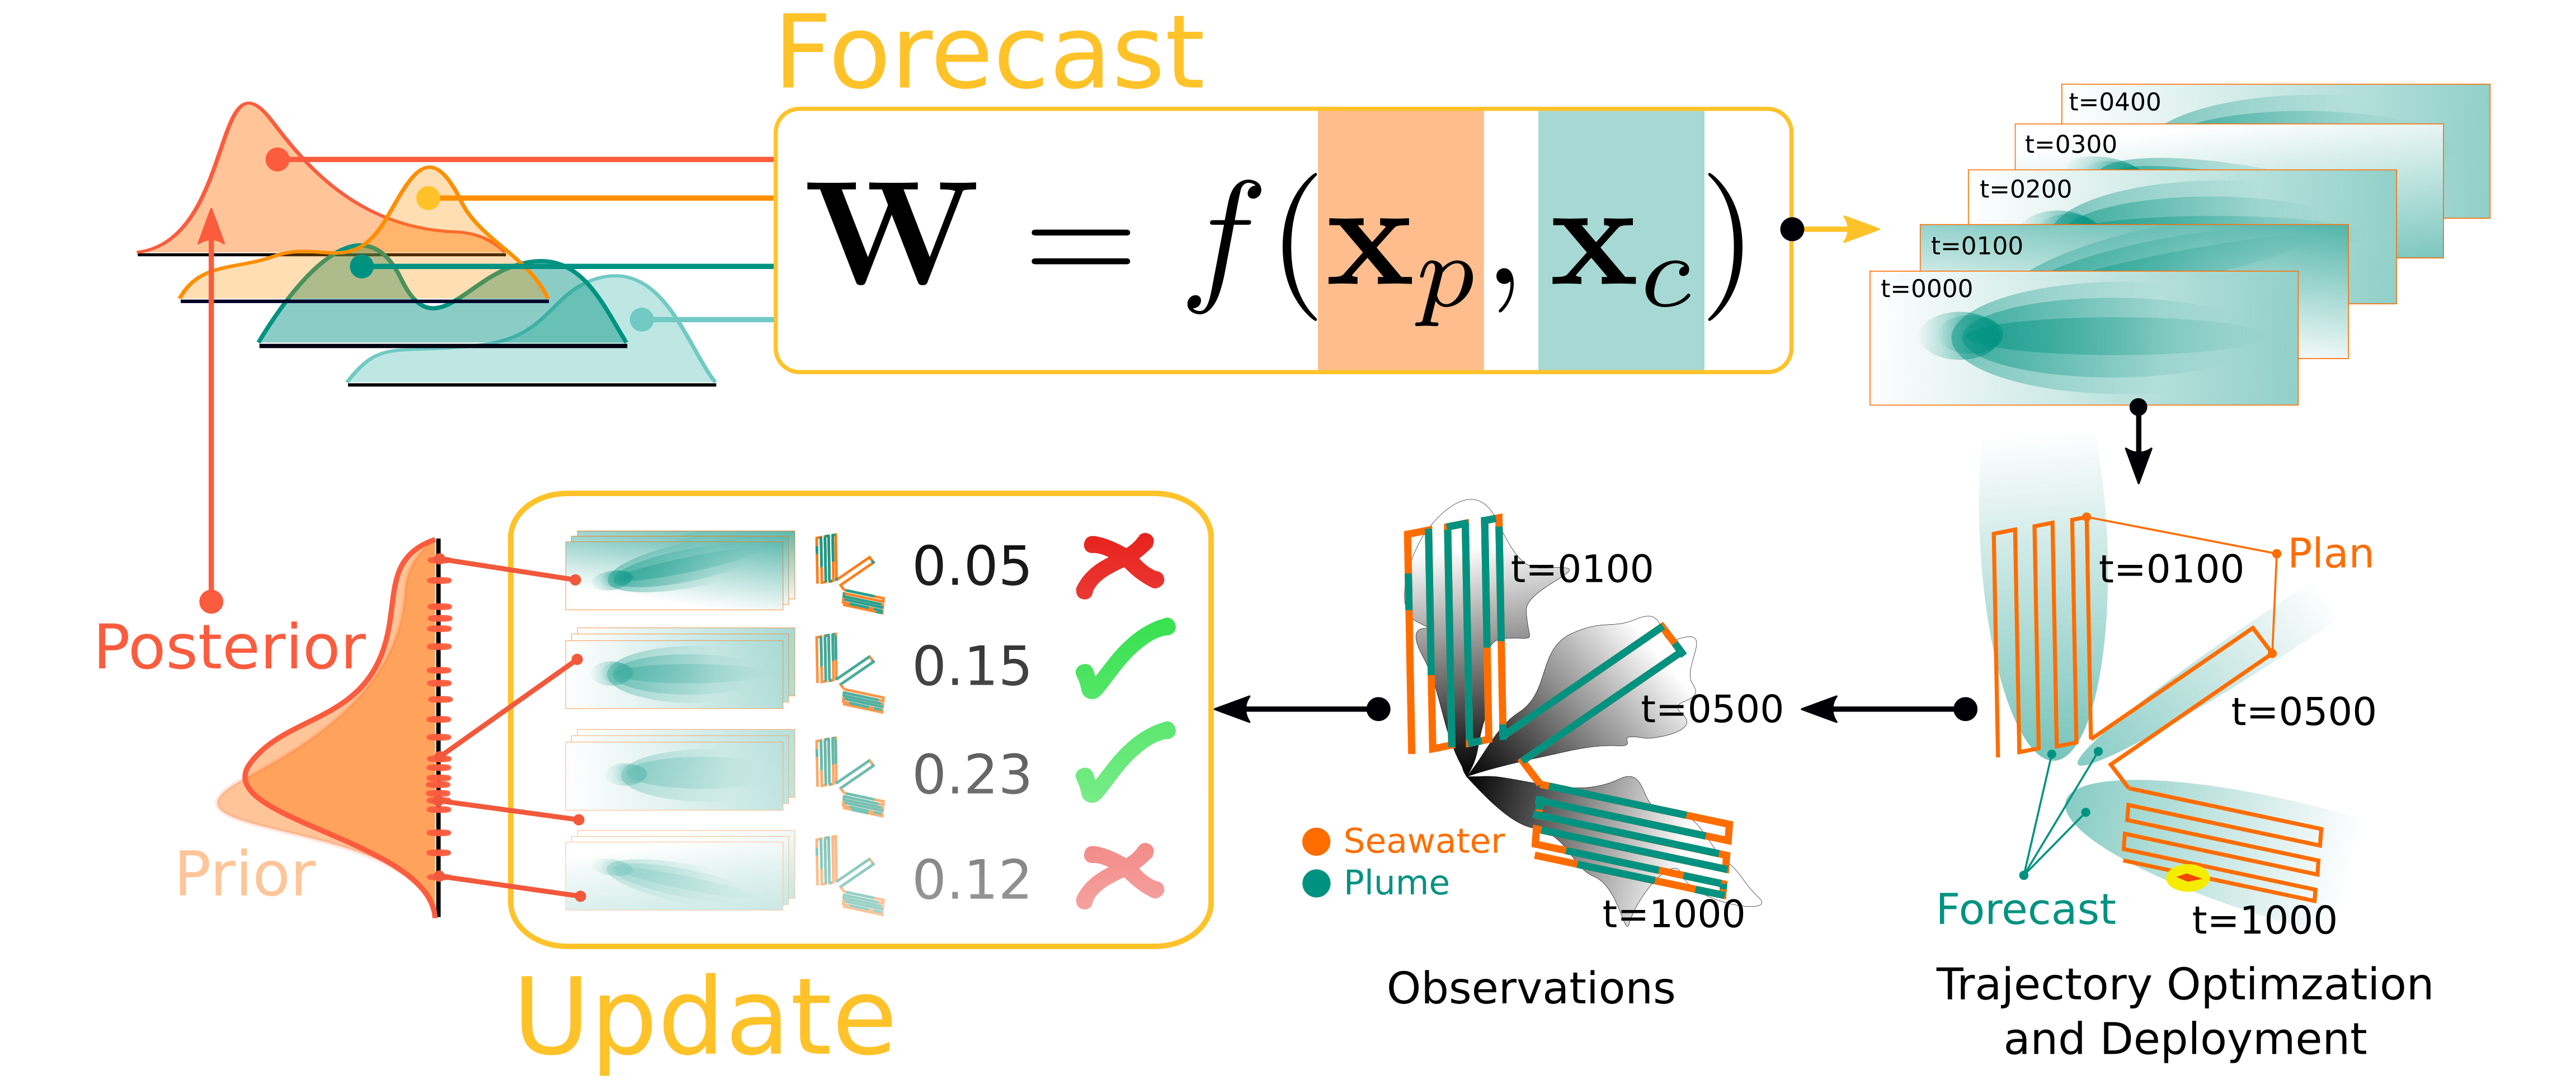
\includegraphics[width=1\columnwidth]{figures/phumes_diagram.png}
    \caption{\textbf{\PHUMES}: \phumes. \PHUMES is a model for forecasting the evolution of a spatiotemporal distribution trained on partial observations. \PHUMES generates forecasts by leveraging an embedded analytical model $f(\cdot, \cdot)$ that approximates the physics-driven evolution of a target distribution. This model is seeded with many samples from distributions placed over initial conditions, physical parameters, or temporal functions (such as $\x_p$ and $\x_c$ here). The composite result of this process is a forecast $\mathbf{W}$ that consists of a mean and variance of phenomenon occupancy in a 3D volume over snapshots of time. This forecast is provided to a trajectory optimizer which sets a deployment trajectory that is executed by a robot. The deployment generates a series of observations, which are then used to update the distributions of the generating distributions via MH-MCMC, which compares the gathered observations with the simulated observations of samples from the generating distributions. The resulting posterior update over the generating distributions is then used for the next planning iteration.}
    \label{fig:phumes}
\end{figure}

\PHUMES consists of two key phases: forecasting (forward simulation) and updating (inverse problem) (\cref{fig:phumes}). In the forecasting step, samples from the distributions of the initial conditions and seawater properties seed the simulator which is solved many times to create a set of plume-envelope samples in the full state space of the target phenomenon (and trajectory optimizer). Time is discretized over domain-specific key points, and any parameters reliant on time are sampled at those discrete points. The set of composite samples at each time is a ``forecast'' that is essentially a series of snapshots of the phenomenon. Precisely, \PHUMES generates a time-indexed $t \in \mathbb{T}$ composite estimate of the distribution of plume fluid in a 3D volume $\overbar{\mathbf{W}}$ by forward simulating time-dependent $M$ samples of the states $x_{p,t}^{(m)} \sim \Pi(\x_p(t))$ and $x_{c,t}^{(m)} \sim \Pi(\x_c(t))$ through the plume simulator $f(\cdot, \cdot)$:

\begin{equation}
    \overbar{\mathbf{W}}_t = \frac{1}{M}\sum_{m=1}^{M} f(x_{p,t}^{(m)}, x_{c,t}^{(m)}) \hspace{1cm} \forall t \in \mathbb{T}.
\end{equation}

The complete forecast $\overbar{\mathbf{W}}_t$ is then used by a trajectory optimizer to approximate the reward function $R([\x_p, \x_c, \x_r]^T, a) = \indic{\texttt{in\_plume}(\x_p, \x_c, \x_r, a)} \approx \indic{\texttt{in\_plume}(\overbar{\mathbf{W}}, a)}$. Equivalently, $\mathbf{W}$ is the robot's belief $b$, and as it consists of a set of samples, any statistical measure (the maximum \emph{a posteriori} estimator (MAP), maximum likelihood estimator (MLE), median, etc.) can be computed. For instance, the variance of the forecast $\mathbf{S}^2_W$ can be computed and used within an information-theoretic reward function (e.g., upper confidence bound), as contingent on the design of a downstream planner. 

After the trajectory optimizer yields a plan, \Sentry is deployed. For a single deployment, upwards of 20,000 observations may be available (each deployment is a minimum of 6 hrs in duration, up to 24 hrs, and sensor measurements are logged at 1 Hz). Using the filter described in \cref{sec:sensor_models}, AUV \Sentry provides observations of binary plume detections. Other sensors of opportunity described in \cref{sec:external_current} provide continuous crossflow magnitude and heading observations. These observations are collated into the sensor model $\Zz$.

At the update step of \PHUMES, the probability distributions over $\x_p$ and $\x_c$ are updated from observations $\Zz$. To find $\Pi(\x_c|\Zz)$ we use GP models for crossflow magnitude and heading as described in \cref{sec:external_current}. The GP kernel parameters are updated using a maximum-likelihood update following typical procedures \autocite{Rasmussen2004}. For $\Pi(\x_p | \Zz)$, we use a random-walk Metropolis-Hastings Markov Chain Monte Carlo (MH-MCMC) method \autocite{metropolis1953equation} to perform the update. Simulations of deployments are generated by solutions to the numerical model $f(\cdot, \cdot)$ seeded with samples from $\x_p$ and $\x_c$. The output of the simulations is directly compared via a likelihood model with the binary observations of plume waters collected by \Sentry. To handle binary measurements, we compute the Brier score \autocite{brier1950verification} over the set of real observations $\Zz$ and set of predictive probabilities $\rho(\cdot)$ of the corresponding simulated observations: $\frac{1}{|\Zz|}\sum_{i=1}^{|\Zz|} (\Zz^{(i)} - \rho(f(x_p, x_c)^{(i)}))^2$. In practice, the predictive probabilities $\rho(\cdot)$ are set according to a false positive rate (the observation is a 1, and the simulation is a 0) and false negative rate (the observation is a 0, and the simulation is a 1) established in consultation with instrument experts on the science team; they are set to 0.1 and 0.3, respectively. With the likelihood model applied, an acceptance criteria of the likelihood and evaluated priors over samples of $\x_p$ is defined, and samples probabilistically accepted or rejected accordingly. As MH-MCMC inference method is a chaining procedure, each sample of $\x_p$ selected is informed by the last, and the cumulative distribution of all accepted samples is guaranteed to converge to the true underlying distribution for each of the elements in $\x_p$ for long enough chains. The posterior distribution $\Pi(\x_p | Z)$ is set as the new sampling distribution for the next forecast to be generated.

While formulated here for a single instance of a plume, it would be trivial to extend \PHUMES for inference over or simulation of the generating parameters of multiple co-located vents by jointly updating parameter vectors for each vent. For scalability, choosing a different chaining procedure to accelerate search through a higher dimensional state space at the update step (for instance, Hamiltonian Monte Carlo\autocite{duane1987hybrid}), could be advantageous.


\subsection{Trajectory Optimization for Path Planning with Fixed Primitives}
\label{sec:to}
Given the hydrothermal plume-charting POMDP model introduced in \cref{sec:problem} and the probabilistic plume predictions generated by \PHUMES, we next consider how to select trajectories for AUV \Sentry that will effectively map the spatiotemporal dynamics of the evolving plume.  We first define a specific planning problem by re-writing the POMDP value function, \cref{eq:value}, in terms of the elements of the hydrothermal POMDP; then, we introduce a sequence of approximations that allow the value function to be feasibly optimized to select high-reward actions.

In each deployment, the planner must select an action in the form of a chained lawnmower trajectory (\cref{fig:traj_opt}). A chained lawnmower is defined by the number, $n \in \Z^+$, of lawnmowers in the chain and the parameters of each individual lawnmower, $\theta_i \in \Theta$ for $i = 1, \dots, n$. These parameters include the height, width, resolution, origin, and orientation of the lawnmower and are sufficient to completely specify a lawnmower trajectory. We define the set $\Theta$ to enforce that the lawnmower trajectories are contained within a pre-defined, rectangular safe region and that each lawnmower obeys a time-based budget constraint. As previously mentioned, this constrained action set is dictated by the operational practices of AUV \Sentry; lawnmower trajectories result largely in \Sentry traveling in straight lines with few, intermittent turns, which is a beneficial paradigm for the navigational sensors used onboard (i.e., acoustic Doppler Velocity Logger (DVL), inertial sensors). Using lawnmower trajectories has the additional benefit of biasing the vehicle to collect spatially diverse datasets that scientists are accustomed to analyzing. 

\begin{figure}[h!]
    \centering
    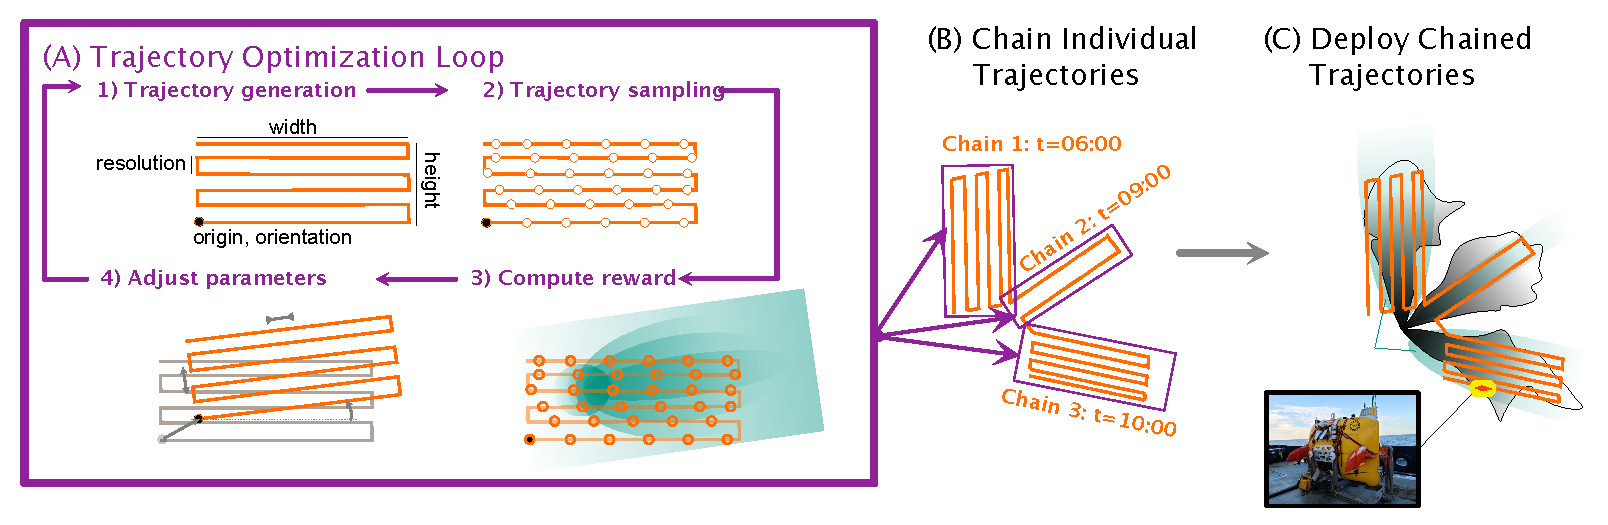
\includegraphics[width=1\columnwidth]{figures/trajectory_optimization.pdf}
    \caption{\textbf{Trajectory Optimization.} The trajectory optimizer leverages the \PHUMES simulator to select high-reward chains of parameterized lawnmower trajectories. (A) The optimization loop for a single lawnmower object, parameterized by height, width, resolution, origin, and orientation. To evaluate the reward of a specific parameter setting, (1) the lawnmower trajectory object is generated using the specified parameters; (2) the trajectory is uniformly sampled along its length to produce a set of sample locations; (3) the reward of those sample locations is computed using the \PHUMES model forecasts of the plume envelope; and (4) the lawnmower parameters are adjusted using gradient-based constrained optimization. (B) This core trajectory optimization loop is used to select parameters for each of a chain of $N$ lawnmowers executed at varying times during the deployment. (C) The chained trajectory is then operationally validated and deployed on AUV \Sentry to collect plume observations.}
    \label{fig:traj_opt}
\end{figure}

We can reformulate the general POMDP value function defined in \cref{eq:value} for the elements of the plume-charting POMDP:
\begin{align}
     V_h^{*}(b) &=  \max_{\{\theta_1, \dots, \theta_n, n \mid \theta_i \in \Theta, n \in \Z^+\}} \mathbb{E}_{[\x_{p}, \x_{c}, \x_{r}]^\top \sim b}[R([\x_{p}, \x_{c}, \x_{r}]^\top, \{\theta_1, \dots, \theta_n\})] \hspace{0.6cm} h \in [0, H-1],
    \label{eq:approx_value}
\end{align}
where each $\theta_i \in \Theta$ parameterizes one of the lawnmower trajectories in a length-$n$ sequence of chained trajectories, and $b$ is the planner's belief about the state of the plume, currents, and robot. In this equation, we see the first of two important planning approximations made by \PHORTEX. As mentioned in \cref{sec:problem}, we set the discount factor $\gamma$ to zero, removing the second, recursive portion of the value function. This approximation significantly reduces the complexity of approximating the POMDP value function, allowing each deployment to be optimized myopically. As deployments of AUV \Sentry are intermittent, time constrained, and start/end on a ship at arbitrary coordinates, the sequence of deployments are largely decoupled; decisions made in one deployment have very little impact on the achievable reward of the next.
%Practically, this approximation only slightly compromises planner performance. Deployments of AUV \Sentry are constrained to start and end at the static location of the ship and the duration of each deployment is fixed by the operational constraints of the scientific expedition. This result of these operational constraints is that sequential deployments are largely decoupled: decisions make in a deployment have very little impact on the achievable reward of the next deployment. 

Solving \cref{eq:approx_value} still involves selecting the number of chains $n$ and the joint optimization of all $n$ lawnmower trajectories in the chain. For a standard parameterization of a lawnmower (height, width, resolution, origin, orientation), this results in a challenging high-dimensional, non-convex, constrained optimization problem in which the dimensionality of the optimization problem changes with the number of lawnmowers selected in the chain. In a typical 15-hour deployment of AUV \Sentry that uses $n=15$, one-hour chained lawnmowers, this results in a 90-dimensional, non-convex joint optimization problem, which must then further be optimized over the number of lawnmowers $n$. Optimization is additionally complicated because evaluating the reward function is computationally expensive, requiring \PHUMES to produce a prediction of plume probability for the locations sampled by a given lawnmower, and by a lack of analytical gradients for the reward function with respect to the lawnmower parameters (gradients are instead computed numerically). 

To simplify the planning problem further to address chaining optimization, we make a second approximation. We assume that the number of chained lawnmowers is given, i.e., $n=N$, and decompose the joint optimization of all chains in a trajectory into $N$-independent optimization problems. This approximation allows us to break a high-dimensional, joint optimization problem into a sequence of much lower-dimensional optimization problems, and is a reasonable approximation if the travel cost between subsequent lawnmowers is not significant. 

The final \PHORTEX value function, with the two approximations we described, is given by the following:
\begin{align}
     V_h^{*}(b) &\approx  \max_{\theta_1 \in \Theta} \dots \max_{\theta_N\in \Theta} \mathbb{E}_{[\x_{p}, \x_{c}, \x_{r}]^\top \sim b}[R([\x_{p}, \x_{c}, \x_{r}]^\top, \{\theta_1, \dots, \theta_N\})] \hspace{0.6cm} h \in [0, H-1].
    \label{eq:approx2_value}
\end{align}
We solve \cref{eq:approx2_value}, which defines multiple, independent, non-convex, constrained optimization problems, using the trust-constrained method in the \texttt{scipy} optimization library for a fixed number of iterations\autocite{conn2000trust}. To evaluate the reward function $R([\x_{p}, \x_{c}, \x_{r}]^\top, \{\theta_1, \dots, \theta_N\})$, we define a trajectory sampler operator $\mathbf{G}: \Theta \to \R^{3 \times k}$ that takes a trajectory parameter vector as input and produces a set of locations in $\R^3$ that will be sampled when the robot executes the trajectory, where $k$ is the number of sampled points. In practice, our trajectory sampler $\mathbf{G}$ produces the lawnmower specified by $\theta$ and then sub-samples uniformly along its length with a fixed spacing. These sample points can then be compared with the plume forecast $\mathbf{W}$ produced by \PHUMES to count the number of sample points that are contained within the inferred plume.


\section{Simulation Experiments}
\label{sec:experiments}
We investigate the performance of \PHORTEX in a simulated environment designed to replicate the field deployment closely. In the simulation, a point robot is tasked with collecting spatially and temporal diverse samples of an advecting plume. Each simulation is a three-dive series in which \PHORTEX starts with an uninformative prior over $\x_p$ and executes an initial naive survey (as would occur in a realistic field scenario), then iteratively updates \PHUMES with collected observations and uses the the trajectory optimizer discussed in \cref{sec:to} to perform two more dives. We perform 10 three-dive simulations for each sampling/planning altitude of \SI{100}{\meter} and \SI{150}{\meter} in the same environment. Each single dive in the three-dive sequence is designed to be 12 hrs of simulated time, on a scale similar to the field deployment missions (over 50 acres, or \SI{0.25}{\kilo\meter\squared}). 

In the simulator, the underlying analytical model in \PHUMES is used to generate a ground-truth environment that closely matches the conditions of the real-world vent using available data. The simulated environment has vent conditions of \SI{300}{\celsius}, 34.608 PSU salinity, \SI{0.8}{\meter\squared} orifice area, and \SI{0.6}{\meter\per\second} initial fluid velocity. The simulated environment sets the mixing coefficients to 0.15 and 0.2 for horizontal and vertical mixing, respectively. The current function sweeps a generated plume from due North to due East over the course of 12 hours of simulation time, and the magnitude cyclically varies with a beginning and end point of \SI{0.11}{\meter\per\second} and minimum at \SI{0.04}{\meter\per\second}. The generating snapshots of the true environment are provided in \cref{fig:sim_env}.

\begin{figure}[h!]
    \centering
    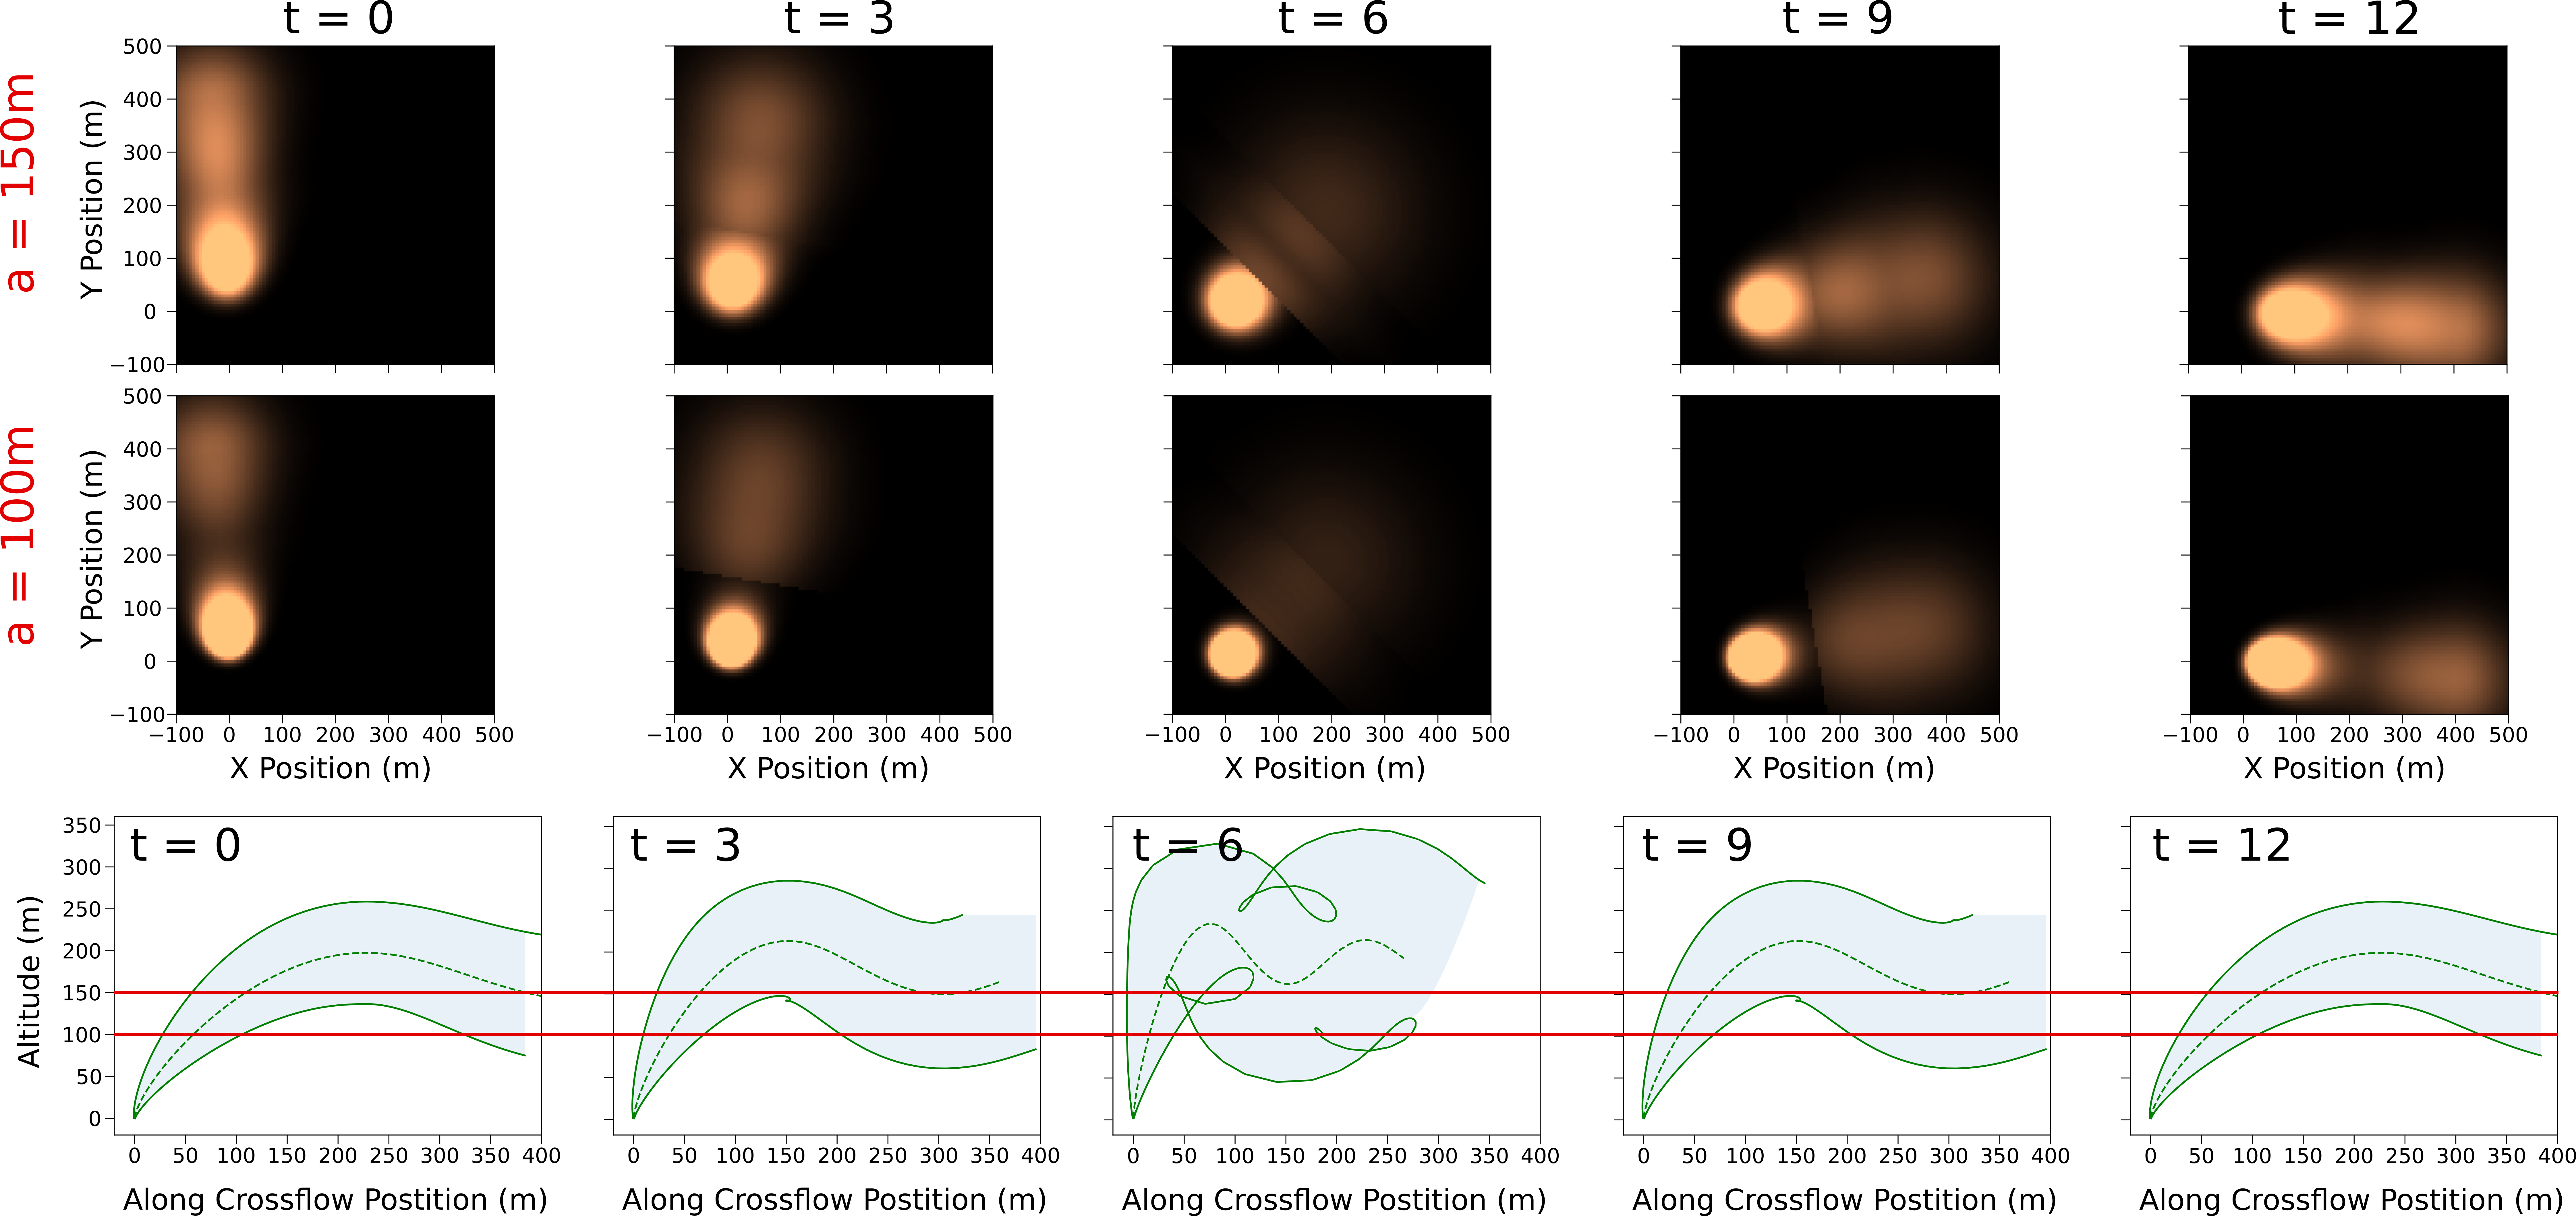
\includegraphics[width=1\columnwidth]{figures/sim_env.png}
    \caption{\textbf{Simulated field trial environment.} Generated environment for simulation trials at different snapshots for altitudes of \SI{100}{\meter} and \SI{150}{\meter}. As the current magnitude and heading changes, the plume expression changes shape and location over 12 hours. Plume intensity is shown in orange in the top plots. The bottom plots show a vertical cross-section of the plume envelope, along the crossflow direction, at different points in the tidal cycle, with the \SI{100}{\meter} and \SI{150}{\meter} horizontal planes marked.}
    \label{fig:sim_env}
\end{figure}

In these experiments, the \PHUMES model must estimate the vent area, vent fluid velocity, and both mixing coefficients from plume observation in the water column, starting with uninformative priors over each of these targets. A noisy current magnitude and heading function is provided to \PHUMES for use in the forecasting and updating step, as would typically be available from sensors of opportunity in the field. For the \PHUMES update, 150 samples from an MH-MCMC chain are used to approximate the posterior distributions over the inference targets (this excludes an initial 50 samples of burn-in). In the first simulated dive, the robot executes a base-case uniformed lawnmower trajectory, placed to intersect the sweeping movement of the current. This trajectory is \SI{15}{\meter} in resolution, and covers a \SI{500}{\meter} by \SI{500}{\meter} area, with no rotation. For the second and third dives, trajectories are optimized using \PHORTEX for the 12-hour mission and consist of four, 3-hour long chained lawnmowers. Each lawnmower in the chain has a fixed resolution of \SI{10}{\meter}, and the height, width, origin, and orientation of each lawnmower are optimized to collect the most reward based on a plume forecast using the maximum \emph{a posteriori} (MAP) sample returned by the \PHUMES model for the four inference targets. The robot travels at approximately \SI{0.5}{\meter\per\second}, collecting binary observations every meter that is traveled. 

\subsection{Evaluation Metrics}
\label{sec:eval_metrics}
The scientific objective of \Sentry in the field trial is to collect observations of a deep-sea hydrothermal plume that have broad coverage in time and space, and thus are useful downstream for characterizing the space-time dynamics of the plume and other related phenomena (i.e., chemical flux, consumption). To evaluate the performance of \PHORTEX for deep-sea plume charting in both simulation and field trials, we introduce three key metrics that measure how well \Sentry collects such samples:
\begin{itemize}
    \item \textbf{Proportion of positive plume observations:} the number of observations collected in a dive that are classified as in-plume by the binary sensor model (\cref{sec:sensor_models}). This metric captures how effectively the robot targeted the plume during a deployment.
    \item \textbf{Spatial utilization:} the most distal plume detection and the ratio between the most distal plume detection and the longest distance that the robot traveled from the plume source. This metric captures the spatial coverage of the plume achieved by the robot and the spatial efficiency of the deployment. For example, if detections were made up to \SI{300}{\meter} away from the vent, but the robot traveled up to \SI{1}{\km} away, then the survey spent too much time outside of the detectable plume region and would not be as effective as a survey that only traveled \SI{200}{\meter} away but stayed well within the detectable plume range. 
    \item \textbf{Temporal utilization:} the proportion of hours in the dive with at least 10\% or more plume detections. This metric quantifies how effective the robot was at \emph{staying in} or \emph{revisiting} the plume over time. Given the long duration of these missions, it is important to use the entire mission window for the task at hand; moreover temporally diverse observations are of scientific interest.
\end{itemize}


% Quality for this task is defined as collecting a high-proportion of in-plume samples over the course of a dive, revisiting a plume over the course of a dive, and collecting in-plume samples as far from the vent as the robot drives. 
\section{\PHORTEX Performance}
\label{sec:phortex_perform}
\cref{fig:sim_traj_example} shows example planned trajectories and \cref{fig:sim_traj_perform} shows the distribution of each of the metrics of interest presented in \cref{sec:eval_metrics}---proportion in plume, spatial utilization, temporal utilization---for the three dives at each altitude tested in the simulated trials. These results demonstrate that the \PHORTEX optimized trajectories significantly outperform the naive baseline, collecting over twice the proportion of samples in-plume, at least doubling the number of hours that the robot spends in a plume, and improving spatial utilization to nearly 100\% from 60-70\%. For analysis of the convergence characteristics of the optimizer, see \cref{app:phortex}. 

\begin{figure}[h!]
    \centering
    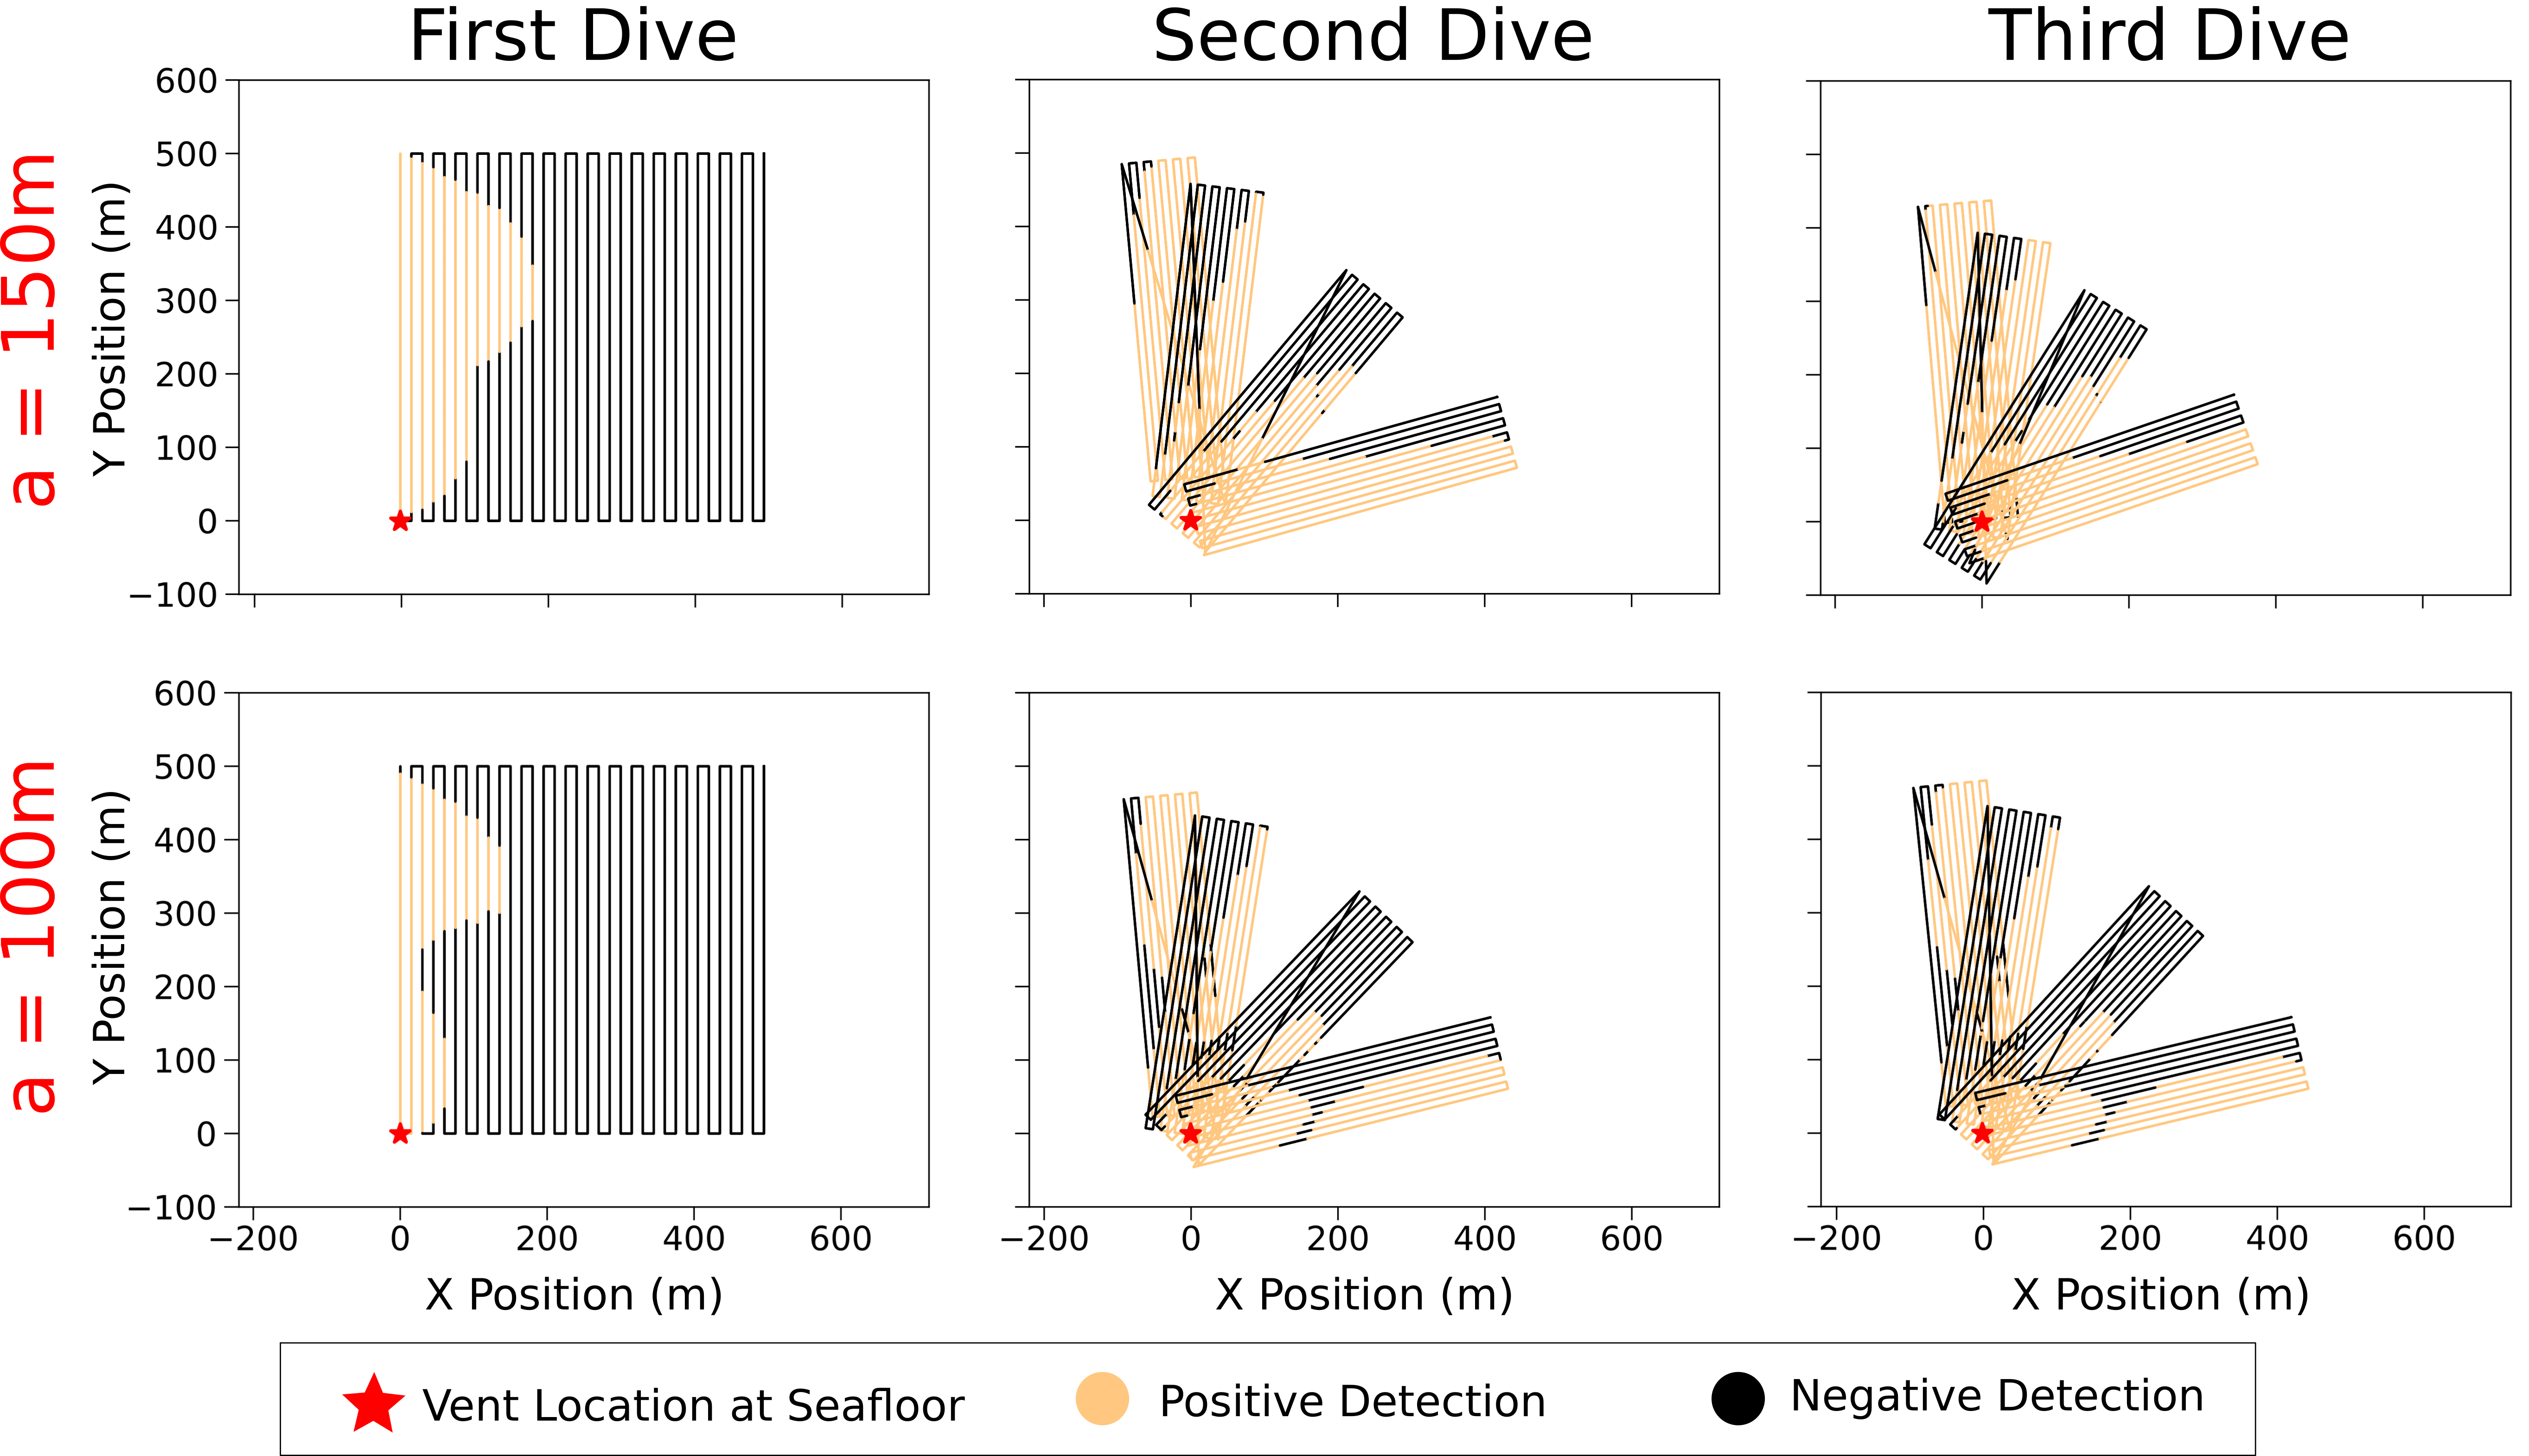
\includegraphics[width=0.85\columnwidth]{figures/sim_traj.png}
    \caption{\textbf{Naive and \PHORTEX-designed trajectories.} Trajectory examples for altitudes of \SI{100}{\meter} and \SI{150}{\meter}. The first dive is always a naive lawnmower; the second and third dive are \PHORTEX designed trajectories. \PHUMES is incrementally trained after each dive on the binary plume detections shown in this plot, which are sampled every meter traveled along the trajectory.}
    \label{fig:sim_traj_example}
\end{figure}

\begin{figure}[h!]
    \centering
    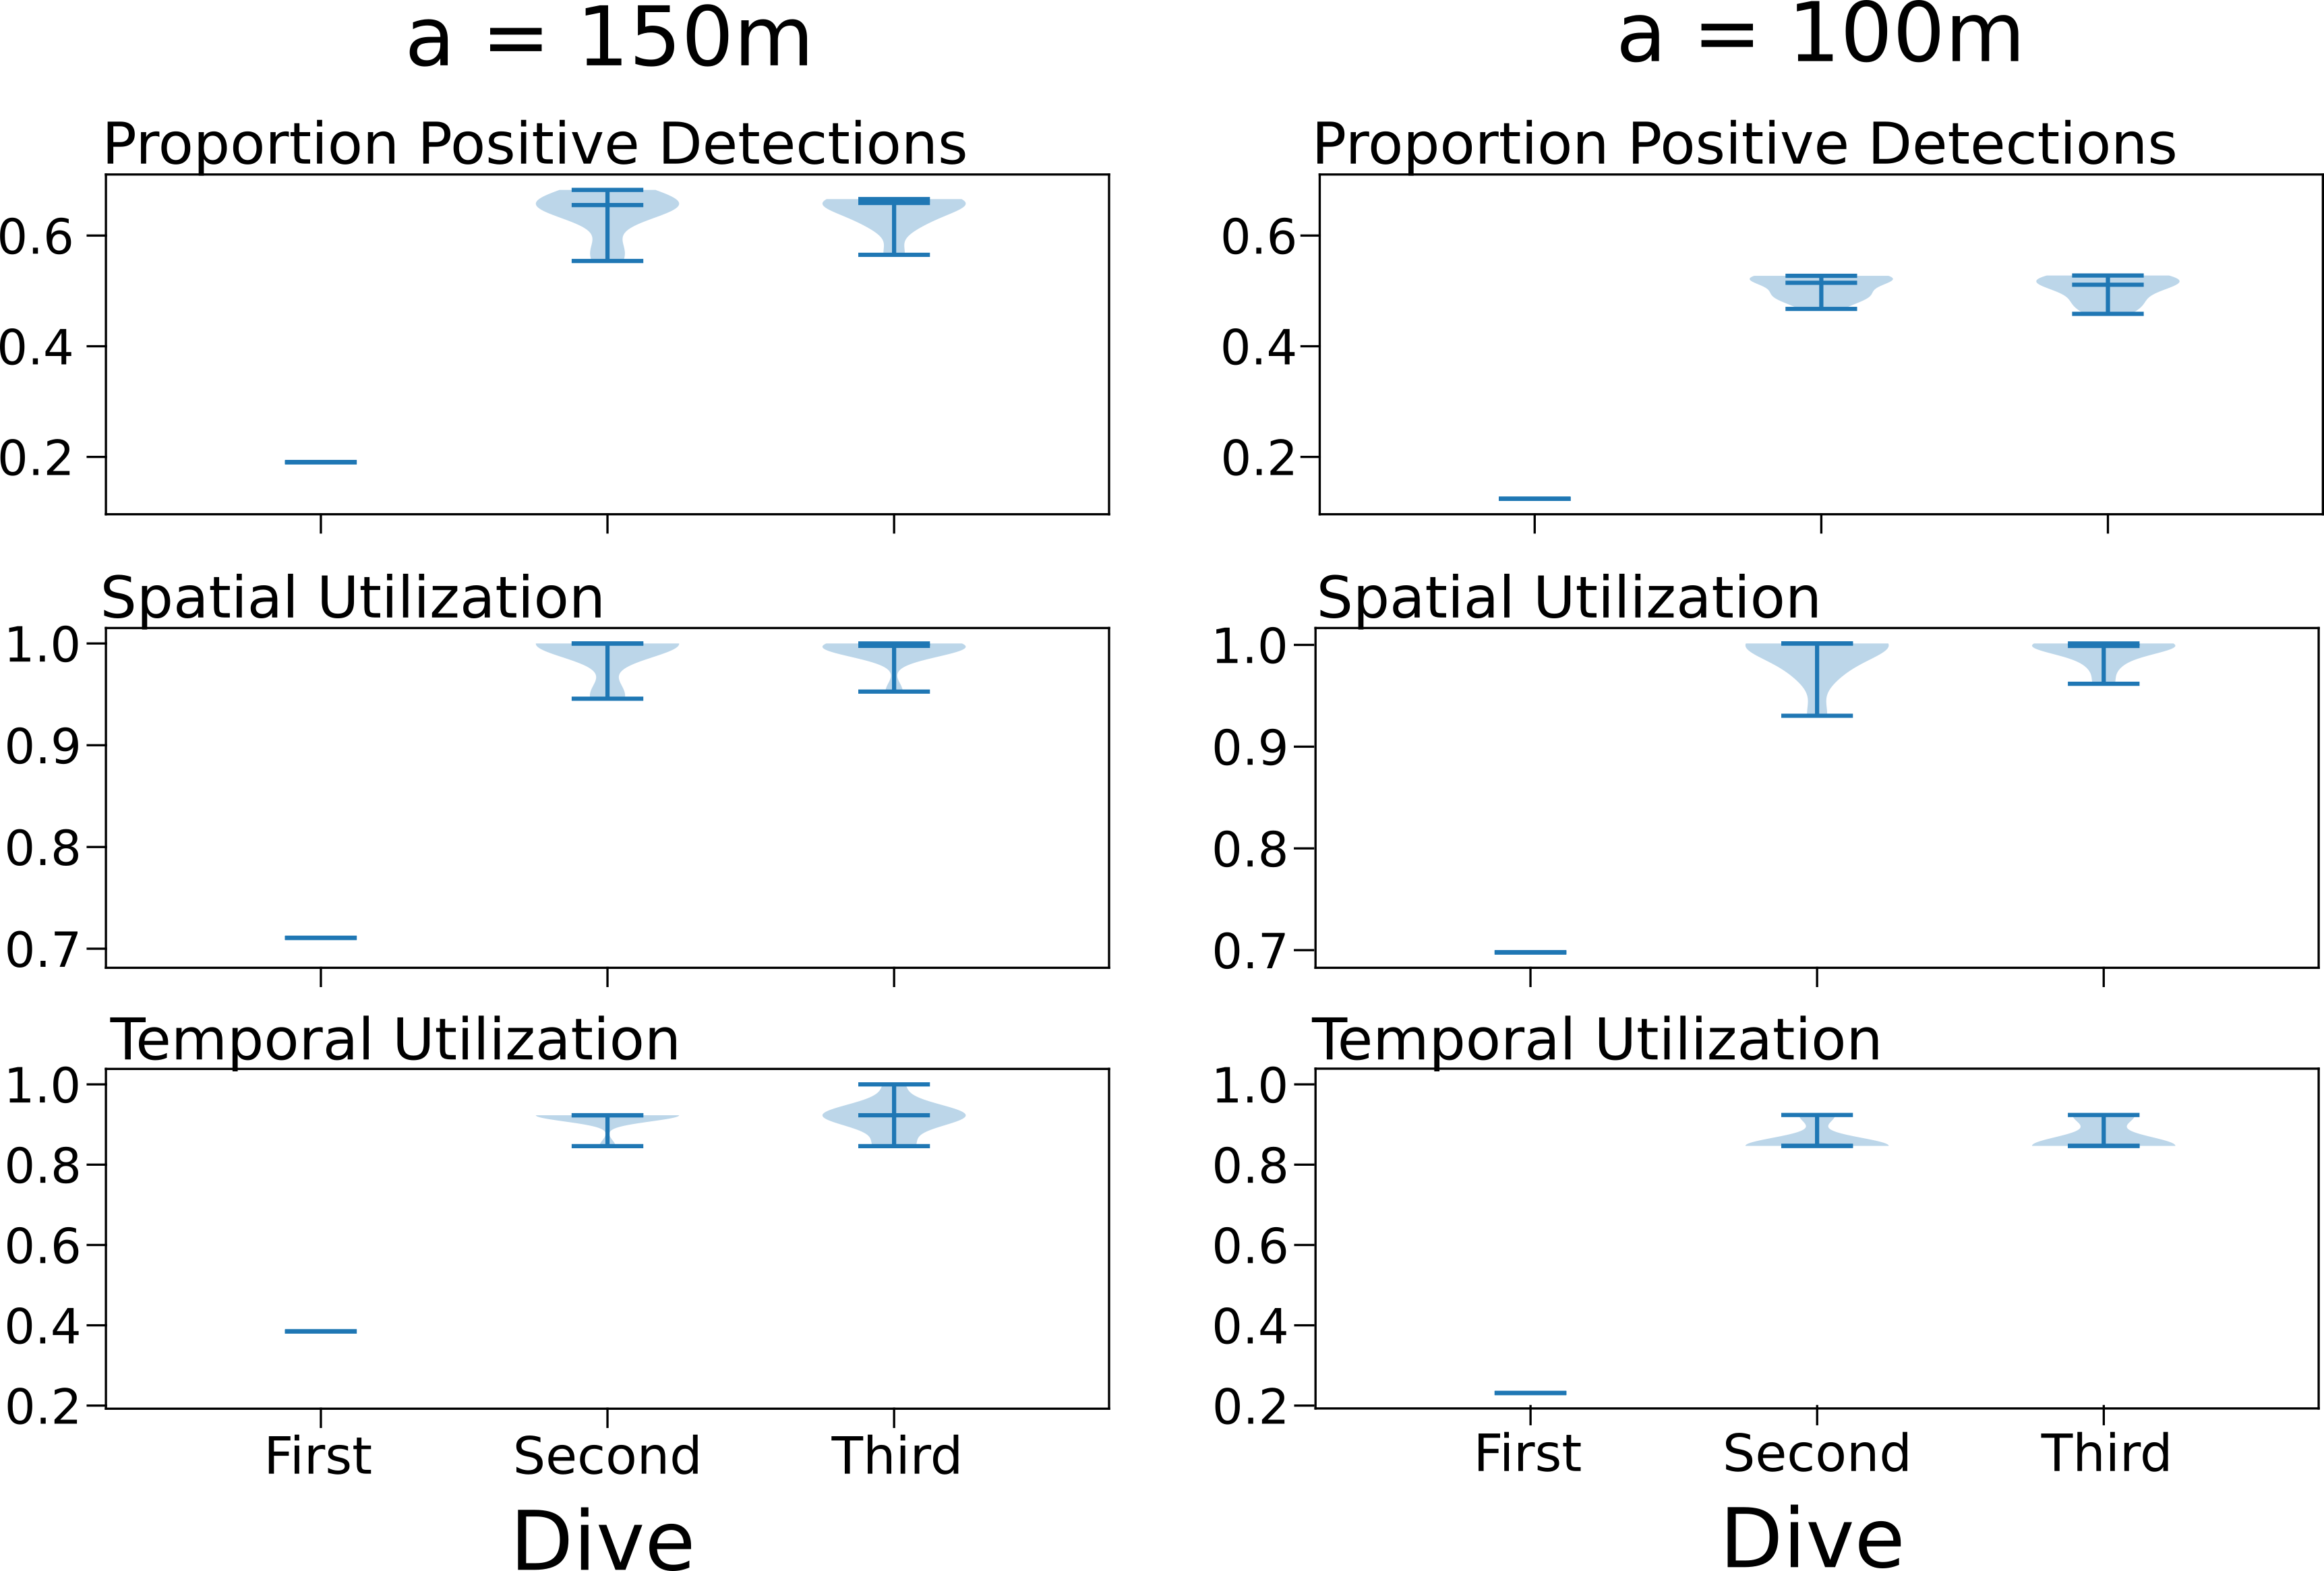
\includegraphics[width=0.75\columnwidth]{figures/sim_traj_performance.png}
    \caption{\textbf{Evaluation of the \PHORTEX trajectories.} The three-dive sequence, consisting of a naive lawnmower followed by two rounds of \PHUMES model training and \PHORTEX trajectory optimization, are evaluated for proportion of positive plume detections, spatial utilization, and temporal utilization (\cref{sec:eval_metrics}). The \PHORTEX-designed dives show a clear improvement in all three metrics, gathering more spatially and temporally diverse observations of the dynamic hydrothermal plume. Iterative rounds of \PHORTEX model-training and trajectory optimization continue to collect a high proportion of scientifically valuable observations.}
    \label{fig:sim_traj_perform}
\end{figure}


\section{\PHUMES Model Validation}
\label{sec:phumes_perform}
The performance of \PHORTEX stays consistently high in the second and third dives, suggesting that \PHUMES quickly learns a sufficient model for planning from the small number of samples collected by the naive trajectories. To further understand the model learned by \PHUMES, we first qualitatively inspect the models learned by \PHUMES in two exemplar trials with data collected at \SI{100}{\meter} and \SI{150}{\meter} altitude during the initial naive survey of the first dive, as presented in \cref{fig:sim_model}. In the naive survey, less than 20\% of all detections are positive detections, and all detections only occur in the first 3 hours of the 12 hour mission. At an altitude of \SI{100}{\meter}, the robot essentially ``skims'' the bottom of the neutrally-buoyant plume; at \SI{150}{\meter}, the robot is consistently within the range of the neutrally-buoyant plume. Despite these altitude differences models learned in this example show remarkably similar characteristics---a predicted centerline no more than \SI{25}{\meter} off from the true environment's centerline, and a width that nearly completely envelopes the true plume distribution, which is promising for the context of planning missions. This is in contrast with an illustrative sample from the uninformative prior, which can arbitrarily produce plume structures that are significantly different in form from the true generating environment. It is also worth noting that despite training data only being available for 3 hours of the 12 hour simulated dive, the predictive quality of the model learned forecasts to an unseen time (t=9hrs) remains high. This largely demonstrates the advantage of using an embedded dynamics model in order to generate predictions of the state space to unseen times.

\begin{figure}[h!]
    \centering
    \includegraphics[width=\columnwidth]{figures/sim_mod.png}
    \caption{\textbf{Illustration of model learning.} Snapshots of the true generating environment are compared with an arbitrary sample from the prior distribution over \PHUMES parameters and the learned models from data collected by naive lawnmowers in both \SI{100}{\meter} and \SI{150}{\meter} simulation trials. In these two exemplar experiments, model learning performance is comparable between the \PHUMES models trained on data from different altitudes. The learned model, in comparison to the baseline sample, demonstrates a lower neutrally buoyant stem height, and is wider, and better explaining the data collected at the two sampling heights. Snapshots at different times show that the learned parameters robustly predict future shapes of the plume, even when trained on partial data available from the naive lawnmowers.}
    \label{fig:sim_model}
\end{figure}

To the quantify performance of the plume forecast generated by the MAP parameter sample after each trial, we compute the intersection over area (IoA) and intersection over union (IoU) between the true environment and each of the learned models after the naive and first \PHORTEX designed dives (\cref{fig:sim_phumes_perform}). A set of 10 parameter samples from the uninformative priors over the inference targets are used to generate an initialization performance distribution to show the breadth of forecast quality before any training. IoA (or recall) provides a number from 0-1 that expresses how many samples in the learned model are shared with the true generating environment. This number does not penalize false positives in the model: a value of 1 implies that all points in the model are contained by the environment, and a 0 implies that there are no points contained in the true environment. IoU (or precision) also provides a number from 0-1 that now penalizes false positives: a value of 1 implies perfect alignment between the model and environment, and a 0 implies no alignment. The comparison of these numbers helps to contextualize the performance of model learning. 

In \cref{fig:sim_phumes_perform}, we see that the learned models have a narrower performance window than the baseline samples, and that they generally exhibit very high IoA (up to 1), and a higher IoU (up to 0.9) than the baseline models (up to 0.75). With a high IoA, we can be confident that the learned models are placing value in areas for which there is plume, and with a higher IoU, we can be confident that the structure of the predicted regions with high value align well with the true environment. Taken together, a very high IoA with medium to high IoU suggest that trajectories planned with the \PHORTEX-trained models are very likely to plan for and successfully execute intersections with the targeted plumes, which is advantageous for our scientific task. We do not see a degradation of performance with different observations available between dives, suggesting that from very little data (a single naive dive), we can train an immediately useful model. Additionally, we note that there is a distinct difference in the distribution shapes of IoA and IoU between the altitudes across these trials. In particular, training from samples at \SI{150}{\meter} appears to be more consistently highly performant (IoA mode is at or near 1; IoU distributions skew towards 0.8) than at the lower altitude, which has a more distributed performance characteristic (with IoA skewed just about 0.8, and IoU centered just above 0.6). This has interesting implications for choosing deployment altitudes in practical missions, within the constraints of robot abilities (for instance, AUV \Sentry cannot swim over a certain altitude and maintain good localization, thus constraining what parts of a plume may be accessible in field deployments). We leave as future work the finer scale characterization of informativeness of different plume regions for model recovery in scientific settings.


\begin{figure}[h!]
    \centering
    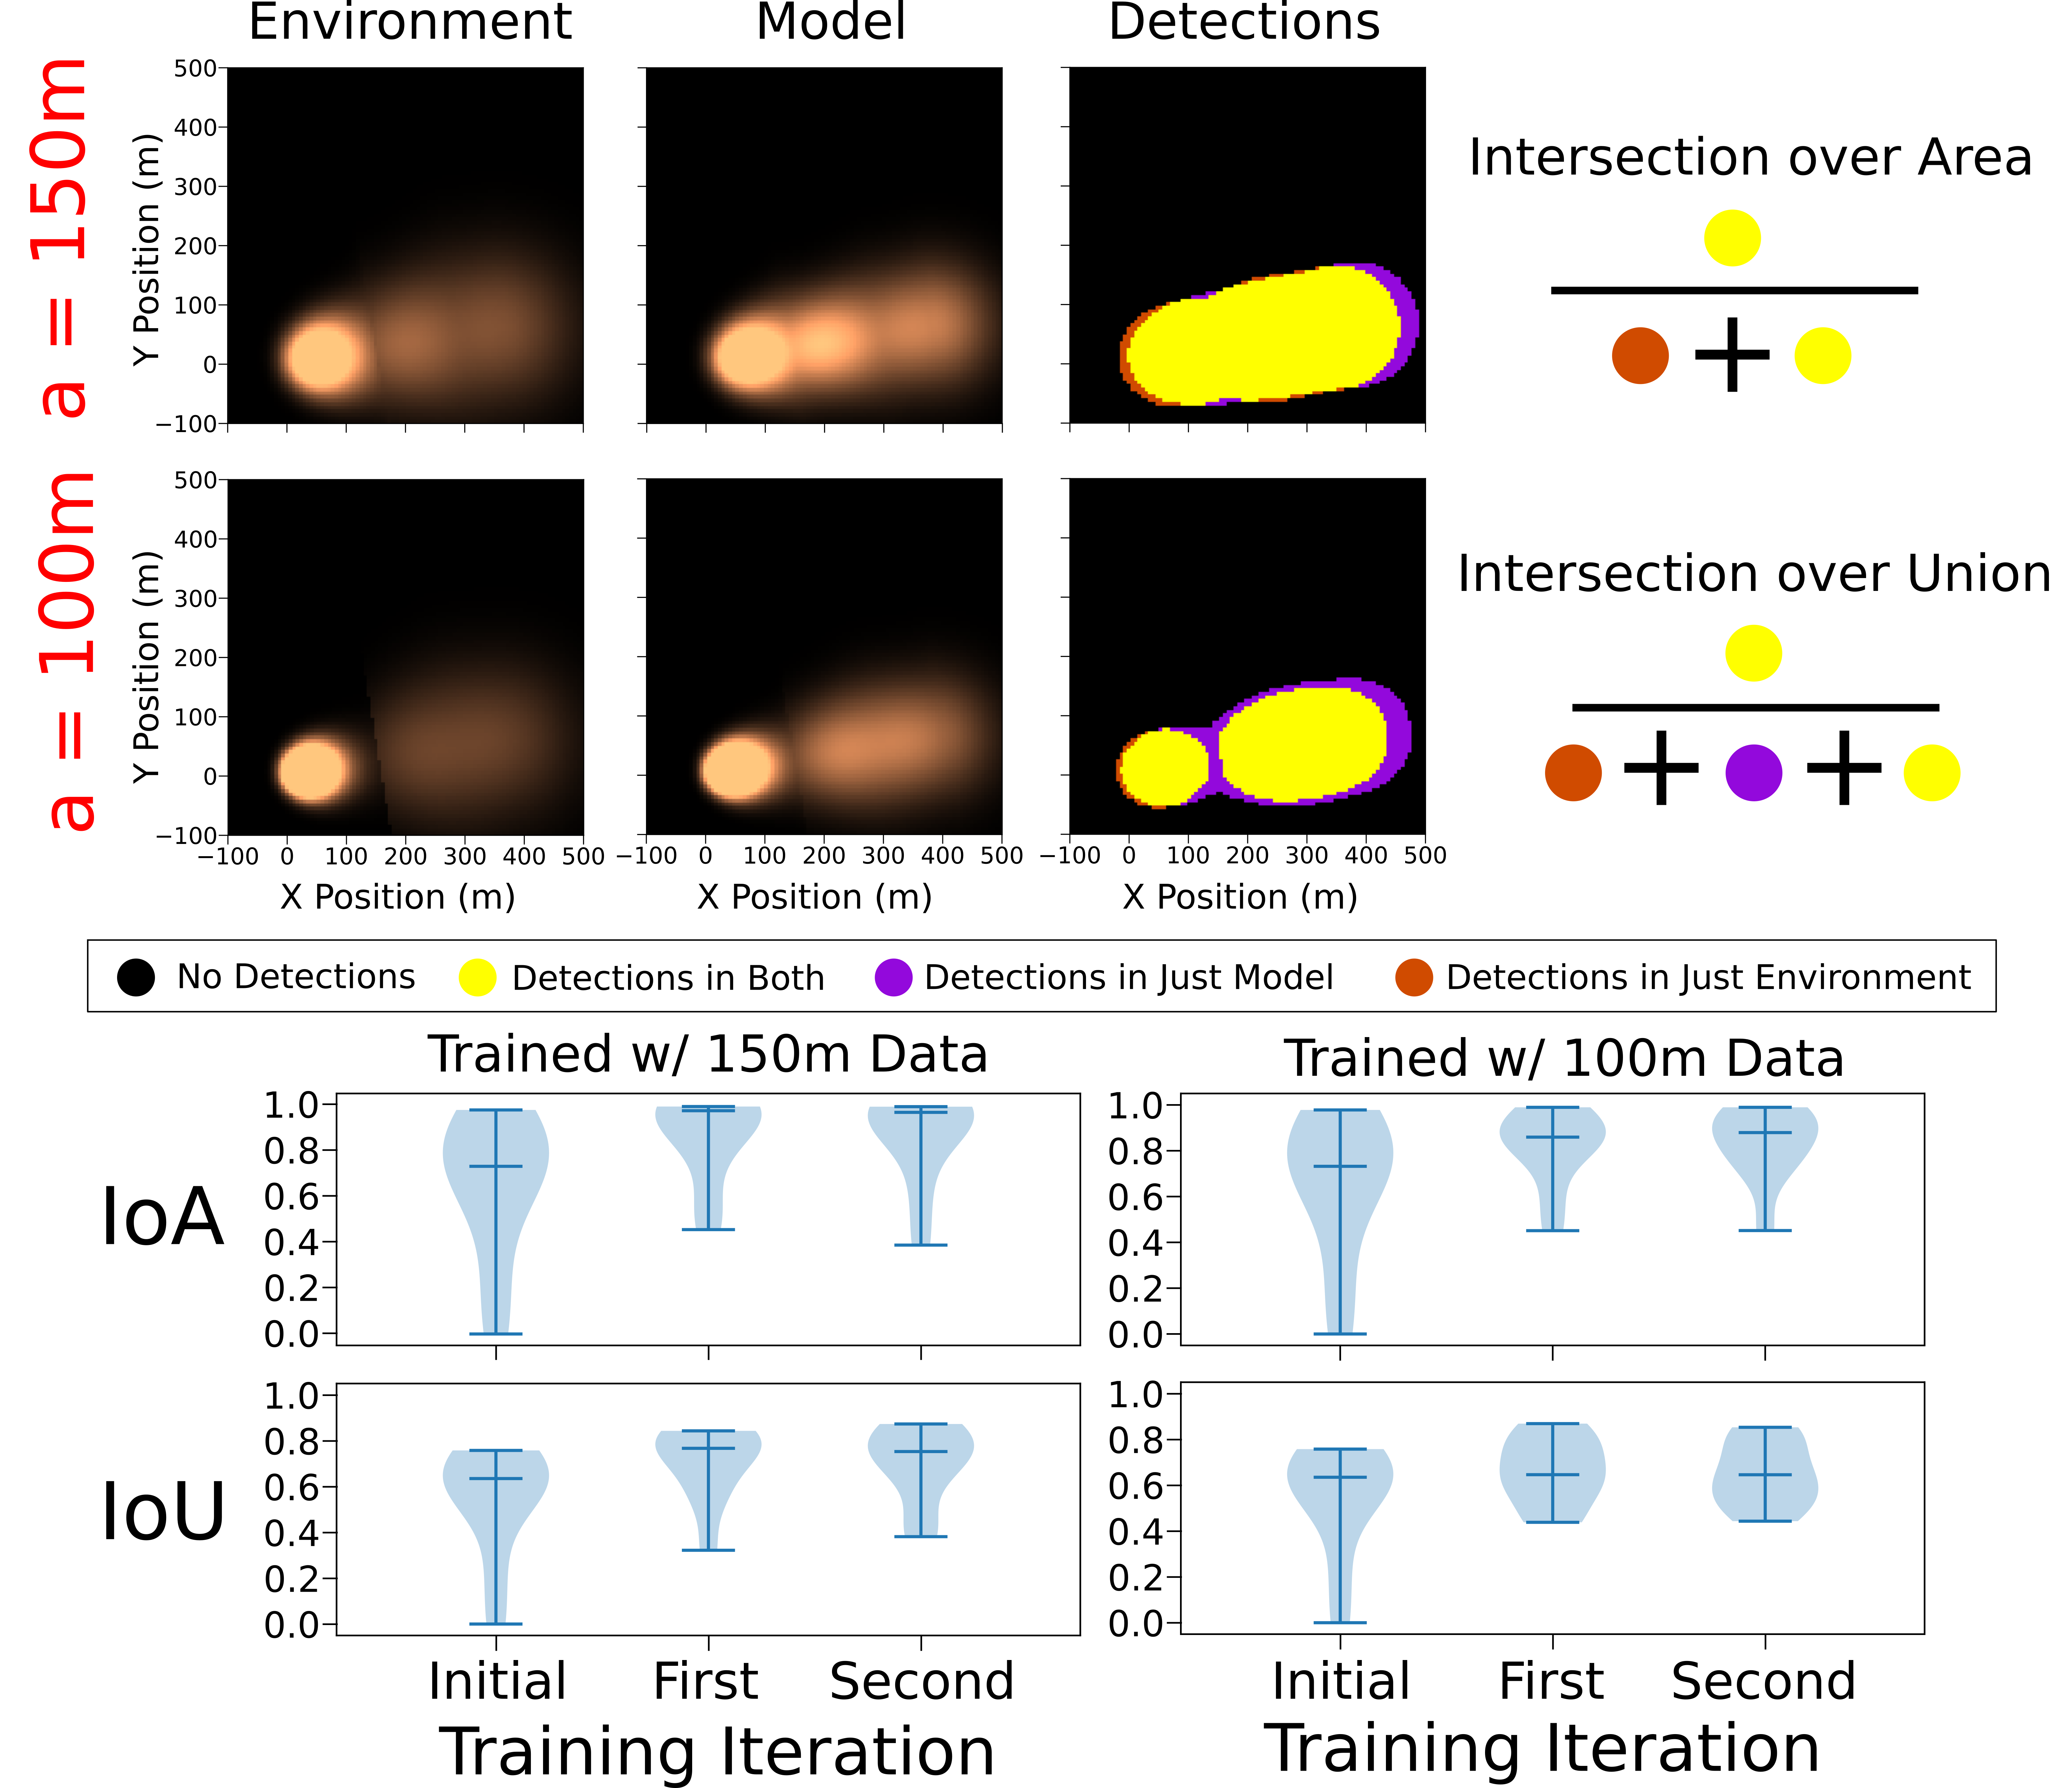
\includegraphics[width=0.9\columnwidth]{figures/sim_mod_performance.png}
    \caption{\textbf{Intersection over Area (IoA) and Intersection over Union (IoU) of trained models.} For each of trials trained from data at \SI{100}{\meter} and \SI{150}{\meter} altitudes, we compute the average IoA and IoU (using the method illustrated at the top) for a set of initial model samples (Initial), \PHUMES trained on the naive dive (First), and \PHUMES trained on the follow-up \PHORTEX-designed dive (Second). In general, we see the each of the iterative trained dives maintains similar performance; with high IoA and medium-to-high IoU that is consistently higher than initialized samples. Trials trained on data from \SI{150}{\meter} tend to have more performant model estimates (IoA near 1, IoU skewed above 0.8) compared to those trials trained on data from \SI{100}{\meter}.}
    \label{fig:sim_phumes_perform}
\end{figure}

In these simulated trials, chain-lengths were dictated by computational constraints placed on the framework to mimic realistic field scenarios, in which only a few hours may be available for plan creation. For more detail on the chaining performance of \PHUMES, see \cref{app:phortex}.

\section{Discussion and Future Work}
\label{sec:future}
Through this simulation work, \PHORTEX is shown to be an autonomy system that can effectively leverage scientific knowledge to enable a deployment-by-deployment mission to chart deep sea hydrothermal plumes. Quantitative gains over typical exploration strategies in terms of number of total in-plume samples, as well as the spatiotemporal diversity of those samples, lends confidence in the ability for this framework to perform in real field settings. As technological advances in robot platforms increase for scientific contexts, advancing \PHORTEX for online settings and adapting multiagent strategies for deep-sea research are attractive next steps. For \PHUMES, improving upon the temporal expressivity of the model presented in this chapter, investigating pre-training opportunities with sophisticated simulators, and adapting state-of-the-art scientific machine learning techniques for a decision-making context, are areas of direct improvement that can be studied. The following sections discuss some of the key challenges in deploying \PHORTEX for hydrothermal plume charting, each of which may be avenues for future work.

\subsection{Temporal Resolution in \PHUMES Forecasts}
The \PHUMES forecast provides a sequence of time-averaged plume ``snapshots'' over which trajectories for a given dive can be planned. By virtue of using the analytical model presented in \cref{sec:phumes}, generating a series of snapshots requires discretizing over time in order to sample a crossflow magnitude and heading, with which the global coordinates of a plume can be computed. This strategy does not capture the effects of advection and mixing on pre-existing (i.e., persistent) plume fluids; the snapshot from $t=0$ does not influence the snapshot of $t=1$ because the persistence of plume fluids generated at $t=0$ are not modeled directly. For the purposes of plume charting in the neutrally-buoyant layer, it could be advantageous to have a more sophisticated model of plume-fluid persistence and/or finer-scale temporal resolution in order to better constrain the spatiotemporal coordinates of a particular observation. For this sophistication to be added, two key innovations would be necessary: a suitable analytical model and a suitable observation scheme.

In settings in which modeling fluid persistence may be useful, a simple advection-diffusion model could be used on-top of the analytical model used in this work to advect neutrally-buoyant fluids between time discretized snapshots. This would be a simple extension that would introduce another uncertain parameter---rate of diffusion---for inference. Another methodology to explore may be integrating other probabilistic tools to estimate unmodeled characteristics of an environment by the analytical model (e.g., learned ``closure'' terms). This may be particularly well-suited in online planning domains, in which forecasts from an analytical model could be used e.g., to set the prior of a GP, and then live observations could be incorporated in real time for course correction while underway. Rather than build upon the model we selected, adapting Gaussian puff models\autocite{ludwig1977simplification} for the deep-sea environment or deriving a minimal set of PDEs to include derivatives in time from full-state models like in~\cite{lavelle2013turbulent} could be fruitful. In this case, to consider persistence requires additionally modeling non-conservative properties of a plume, such as biological nutrient consumption or particulate deposition. As designing analytical models of these phenomenon is an active area of research, it is obvious that working with domain experts to formulate the right physically-informed model for \PHUMES is critical.

The observation scheme for a particular implementation has considerable impact on the sophistication of the inference that can be accomplished. In hydrothermal plume charting, there are heuristics for particular sensors that we employed to create a simplified binary data product; however a similar scheme could be used to develop a more continuous measure of the ``plume-quality'' of a particular water sample, or a learned sensor could be developed which could potentially create a more expressive data product. One of the challenges with environmental domains is the access to enough training data to create such learned sensors. But perhaps the larger challenge is simply the quality of the data available at large---much of the carbonate and other biogeochemical systems of environmental interest have either a limited or nonexistent selection of (\emph{in situ}) sensors available to measure them. Of the sensors that exist, particularly for deep-sea work, the time-response of gas sensors is on the order of half-an-hour or longer (in this work, we made use of experimental sensors in active development with faster response times suitable for mobile AUVs). As the sophistication of sensing equipment improves, so too will the inference abilities of decision-making systems like \PHORTEX. 

\paragraph{Lawnmower Trajectories for Dynamic Phenomena}
Lawnmowers and other parameterized trajectories are the foundation of many field robotics deployments. When used to study spatially-distributed static phenomena, lawnmower trajectories produce intuitive, uniform-coverage maps that are easily interpreted by scientists and domain experts. Studying dynamic phenomena, on the other hand, with lawnmower trajectories can lead to highly counter-intuitive and uninterpretable results. For example, the positive plume detections returned by the standard lawnmower trajectory in \cref{fig:sim_traj_example} only barely resemble the underlying dynamic plume. \PHORTEX demonstrates that lawnmower trajectories can still be useful for characterizing dynamic phenomena, when used in combination with probabilistic forecasting models and optimization techniques. However, these methods introduce their own challenges. In \PHORTEX, evaluating the reward of a lawnmower trajectory requires generating the trajectory from parameters, sub-sampling that trajectory, and then using the \PHUMES model to predict the plume snapshot for a specific point in time and space. Each of these steps can be computationally expensive. To increase the efficiency of the trajectory optimizer during field deployments, we discretized time coarsely and only generated the MAP \PHUMES snapshot once for each lawnmower in the chained trajectories (at the start time of the lawnmower). This substantially improved the speed of the planner, at a loss of targeting accuracy for the moving plume. Developing efficient and accurate techniques that can optimize parameterized trajectories, such as lawnmowers, for dynamic environments is an imperative step in effectively studying spatiotemporal phenomena with mobile robots.

\paragraph{Ambiguity Challenges in Inference}
Estimating the plume parameters $\x_p$ for deep-sea hydrothermal plumes requires solving an ill-posed inverse problem. The relationship between fluid exit velocity and vent area are significantly entwined in the analytical model proposed in ~\cref{sec:phumes} via \cref{eq:heat_flux}-\cref{eq:buoyancy_flux}. There are countably infinite solutions on the two-dimensional manifold describing this relationship for a single target flux value. Ambiguity in inverse problems is a classical problem in numerical methods, and not easily resolved without setting strong assumptions (i.e., fixing an unknown parameter) or changing the experimental procedure (i.e., collecting more/different types of data). For the purposes of robot trajectory planning, parameter ambiguity is not \emph{necessarily} a problem, as long as the resulting model is sufficient for predicting the plume envelope to strategically place the robot. However, resolving this ambiguity may be important in settings in which the posterior estimates trained by \PHUMES are used as a scientific data product in of themselves to make claims about a target environment. To make \PHUMES a useful science product (and not just a useful model for planning trajectories), further development that investigates the calibration of uncertainty in posterior estimates and considers possible modifications to the experimental procedure, would be necessary. 


\section{Conclusion}
\label{sec:conclusion}
This chapter presents \PHORTEX: \phortex. \PHORTEX is an autonomy stack that plans long-horizon, fixed trajectories to target a partially observable spatiotemporal phenomena by leveraging physics-based dynamical models and Bayesian inference. \PHORTEX is motivated by the problem of deep-sea hydrothermal plume charting with AUV \Sentry, which requires an autonomous agent to map a spatiotemporally evolving plume structure without using underway adaptive capabilities. With these operational constraints in mind, \PHORTEX implements a ``deployment-by-deployment'' autonomy loop (model update, trajectory design, and trajectory execution) for field operations. At its core, \PHORTEX consists of a trajectory optimizer and the \PHUMES model. The \PHUMES model uses an embedded plume physics simulator to solve a Bayesian inverse problem and forecasts discrete snapshots of 3D plume volumes in time. The trajectory optimizer plans parameterized, chained lawnmower-pattern primitives using \PHUMES forecasts to create multi-hour trajectories that maximize expected plume detections. These trajectories are then validated using \Sentry safety checks and deployed. 

We validated \PHORTEX in simulation, showing that \PHORTEX-designed trajectories can yield obvious gains over naive lawnmower approaches across metrics including total proportion of in-plume samples, and spatiotemporal diversity of those samples. We additionally demonstrated that trained \PHUMES models yield insightful and physically-realistic forecasts that closely match an underlying environment, even in times or places that are not directly observed by the robot while collecting training data; particularly we show that \PHUMES converges to this good estimate in as little as a single dive in the simulated scenario, agnostic of deployment altitude.

Understanding our dynamic and changing environment is a pressing societal challenge, and algorithmic development in the service of expeditionary science presents many compelling challenges in scientific machine learning, decision-making and the integration of research and practice for field robotics. The contribution of this work is to demonstrate the utility of incorporating domain-specific knowledge into autonomy frameworks for science, provide an example of how scientific knowledge and operational constraints can be formulated into a sophisticated (and deployable) autonomy stack, and demonstrate the scientific value of such an approach on the real expeditionary science problem of deep-sea hydrothermal plume charting.
